\documentclass[10pt]{article}
\usepackage{times}
\usepackage{fullpage}
\usepackage[left=0.8in,top=0.8in,right=0.8in,bottom=0.8in,nohead,foot=0.5in]{geometry}
\usepackage{listings}
\usepackage{balance}
\usepackage{graphicx} 
\usepackage{nameref}
\usepackage[margin=10pt,font=small,singlelinecheck=false,labelsep=period]{caption}
\usepackage{titlesec}
\titleformat{\section}{\large\bfseries}{\thesection}{1em}{}

\usepackage{color}

\lstdefinelanguage{chapel}
  {
    morekeywords={
      and, array, atomic,
      begin, bool, break,
      call, class, cobegin, complex, config, const, constructor, continue,
      def, distribute, do, domain,
      else, enum, except,
      for, forall,
      goto,
      if, imag, implements, in, int, inout, _invariant, iterator,
      let, like,
      module,
      nil, not,
      on, or, ordered, otherwise, out,
      param, _private, private, public,
      real, record, _release, repeat, return,
      select, serial, single, subtype, sync
      then, to, type, typeselect,
      uint, union, until, _unordered,
      var, _view,
      when, where, while, with,
      yield
    },
    sensitive=false,
    mathescape=false,
    morecomment=[l]{//},
    morecomment=[s]{/*}{*/},
    morestring=[b]",
}

\lstset{
    basicstyle=\footnotesize\tt,
    keywordstyle=\bf,
    commentstyle=\em,
    showstringspaces=false,
    flexiblecolumns=false,
    numbers=left,
    numbersep=5pt,
    numberstyle=\tiny,
    numberblanklines=false,
    stepnumber=0
  }

\newcommand{\chpl}[1]{\lstinline[language=chapel,basicstyle=\normalsize\tt,keywordstyle=]!#1!}

\lstnewenvironment{chapel}{\lstset{language=chapel,xleftmargin=2pc}}{}


\newcommand{\ie}{\emph{i.e.}}
\newcommand{\eg}{\emph{e.g.}}

\newfont{\affaddr}{phvr at 10pt}
\newfont{\affaddrit}{phvro at 10pt}

\setlength{\parskip}{5pt}
\setlength{\parindent}{0pt}

\title{Chapel Compiler Overview}

\author{Steve Deitz}

\date{June, 2010}

\begin{document}

\maketitle

\begin{quote}
\footnotesize
{\bf Disclaimer.}  This document attempts to explain how the
Chapel compiler works.  It is not always complete and correct.
\end{quote}

{
  \footnotesize
  \tableofcontents
}

\section{Introduction}

This document contains rough notes about the state of the compiler in
June of 2010, sometimes updated with more recent developments.
It is subdivided into three sections.
Section~\ref{sec:ast} describes the intermediate representation,
sometimes referred to as the AST.  Section~\ref{sec:passes} describes
the passes and assumptions that may be made about the AST before and
after the various passes.  Section~\ref{sec:misc} covers miscellaneous
topics.

This document assumes the reader has excellent familiarity with the
Chapel language and understands general compiler construction principles.

\section{Intermediate Representation}
\label{sec:ast}

The intermediate representation (IR), alternatively called the AST, is
a graph-like structure defined by instances of subclasses of the
Symbol, Type, and Expr classes (which are themselves subclasses of the
BaseAST class).  This representation is used throughout the entire
compilation process, though assumptions on its structure change.  (For
example, after normalization, CallExprs will not be nested with the
exception of a CallExpr that represents the MOVE primitive (C
assignment).)  The BaseAST, Symbol, Type, and Expr classes are never
instantiated.

This graph is rooted at the module \cc{rootModule} which contains DefExprs
of all the modules in the program, as well as literals and other
global entities.

Nodes in the representation can also be accessed via global vectors of
each node type.  These vectors are named as \cc{gASTs} where \cc{AST}
is a particular AST node type.  For example, \cc{gFnSymbols} is a
vector of all of the functions in a program, nested or not.  Newly
constructed nodes are automatically added to these vectors by their
constructors.  Between passes, these vectors are pruned of all AST
nodes that are not part of the IR (part of the graph).

Three vectors of modules also capture the modules that make up the
AST.  The vector \cc{allModules} is a vector of all the modules, and
is probably identical to \cc{gModuleSymbols}.  The vector
\cc{userModules} contains all of the user modules.  For debug
purposes, this is useful for looking at the test code in question.
The vector \cc{mainModules} contains all of the main modules.  See
Section~\ref{sec:modulesymbol} for more information on modules.

\subsection{BaseAST}

Every node in the AST is a subclass of BaseAST.  The BaseAST class
contains three fields:
\begin{itemize}
\item \cc{AstTag astTag} is an enumeration value used to identify a
  node's dynamic type. It corresponds directly to the specific class
  that the node is an instance of.  \cc{astTag} is accessed via macros
  \cc{isAST} and \cc{toAST}, where \cc{AST} is replaced by a node
  type.  \cc{isAST} checks if a node is a particular type.  \cc{toAST}
  casts a node to such a type or produces NULL if it is not exactly
  that type.  This cast mechanism is used instead of C++'s
  \cc{dynamic_cast} mechanism.

\item \cc{int id} is a unique integer assigned during construction.
  This is useful for debugging as each AST node will be numbered based
  on the order of construction.  These numbers start at 1.  During
  debugging with gdb via the --gdb flag, you can use the call \cc{aid(ID)}
  to get a pointer to the AST node for the given \cc{ID}.

\item \cc{int lineno} stores the line number of the Chapel code that
  this AST node originated from.  During parsing, this field is set
  based on YACC state.  Afterwards, these numbers are set based on the
  global variable \cc{currentLineno}.  This line number can be changed
  using the macro \cc{SET_LINENO(ast)} which will set the global line
  number to the line number associated with a given AST node.  Thus,
  for example, if you are adding a compiler-inserted CallExpr before
  an existing CallExpr in the AST, you can set the global line number
  to that of the existing CallExpr, and the new compiler-inserted AST
  nodes will use the same line number.
\end{itemize}

As a note for improvement, our line numbers are often incorrectly
reported.  If \cc{SET_LINENO} were used more consistently, this would
not be the case.  One way to improve things would be to generate an
internal error if \cc{SET_LINENO} were not used correctly.  To do
this, we would want to unset the line number somehow.  We could do
this with an \cc{UNSET_LINENO} macro or we could make the
\cc{SET_LINENO} macro require us to open a scope.  Then when we leave
this scope, we could set the current line number back to what it was
before we opened this scope (and unset at the outermost level).

\subsection{Symbol}

The Symbol group of AST nodes derive from the class Symbol.
Variables, constants, parameters, literals, arguments, fields, types,
enumeration symbols, modules, and labels are all represented by
symbols in the AST.

The fields in Symbol are:
\begin{itemize}
\item \cc{const char* name} stores the Chapel name of the symbol.
  This is used during scope resolution and function resolution to
  resolve unresolved symbol uses (UnresolvedSymExprs).  Comparing this
  field does not require a string comparison as it is canonicalized
  (see note on strings in Section~\ref{sec:strings}).
\item \cc{const char* cname} stores the name that we will generate in
  C.  This name is sometimes set during compilation to improve the
  readability of the generated code.  During the codegen pass, we
  legalize these names and mangle them as necessary.  Like \cc{name}, comparing this
  field does not require a string comparison as it is canonicalized
  (see note on strings in Section~\ref{sec:strings}).
\item \cc{Type* type} stores the resolved type of variables,
  arguments, and fields.  This is generally set during function
  resolution when types are resolved.  Before such resolution, the
  type \cc{dtUnknown} is used.
\item \cc{DefExpr* defPoint} points to a \cc{DefExpr}, the expression
  hook in the AST.  Every symbol has a DefExpr that connects the
  symbol to the AST.  The symbol can also show up in the AST via the
  expression \cc{SymExpr}.  These account for both defs (writes to the
  symbols) and uses (reads of the symbols).
\item \cc{std::bitset<NUM_FLAGS> flags} is a bit vector of flags
  (referred to as pragmas when they appear in Chapel code).  Flags are
  associated only with symbols.  See Section~\ref{sec:flags} for more
  information about flags.
\end{itemize}

The subclasses of Symbol include the following:
\begin{itemize}
\item VarSymbol (Section~\ref{sec:varsymbol})
\item ArgSymbol (Section~\ref{sec:argsymbol})
\item TypeSymbol (Section~\ref{sec:typesymbol})
\item FnSymbol (Section~\ref{sec:fnsymbol})
\item EnumSymbol (Section~\ref{sec:enumsymbol})
\item LabelSymbol (Section~\ref{sec:labelsymbol})
\item ModuleSymbol (Section~\ref{sec:modulesymbol})
\end{itemize}

\subsubsection{VarSymbol}
\label{sec:varsymbol}

The VarSymbol class represents variables, including both global
variables (in a module) and local variables (in a function).  The
VarSymbol is also used for fields (in a type).

The constness of a variable is handled via a flag, so constants and
parameters (compile-time constants) are represented by VarSymbol
objects as well.

VarSymbols are also used to represent literals (e.g. the integer
constant 1) using the field \cc{immediate} (see below).  The
representation of immediates is code that came from IF1, an iterative
flow analysis engine.  The \cc{name} of such a VarSymbol is
automatically generated by the compiler.

The fields of VarSymbol include the following:
\begin{itemize}
\item \cc{Immediate* immediate} stores a representation of a literal symbol.
\end{itemize}

\subsubsection{ArgSymbol}
\label{sec:argsymbol}

The ArgSymbol class is used to represent the formal arguments of
functions.  The fields of the ArgSymbol include the following:
\begin{itemize}
\item \cc{IntentTag intent} stores the specified intent of the
  argument.  This can be blank, in, inout, out, or const.  Note that
  \cc{INTENT_REF} does not appear to be used and probably predates the
  introduction of reference types.  The intent field also marks
  generics via parameter and type intent arguments.  The intent field
  is largely ignored after function resolution, which is to say that
  the functionality of the intent has been folded into the
  representation without it.  Thus if the intent were inout, then a
  copy in and a copy out (via assignment and/or a move primitive)
  would have been added to the AST.
\item \cc{BlockStmt* typeExpr} stores the type of the argument as it
  is parsed in.  This specified type is resolved during function
  resolution when the \cc{type} field is set.  After the \cc{type}
  field is set, this field is ignored.
\item \cc{BlockStmt* defaultExpr} stores the expression specified as a
  default for the argument (what is used if no actual is specified).
  The default expression is folded into the AST during function
  resolution by creating a default wrapper function.
\item \cc{BlockStmt* variableExpr} stores the expression specified
  after an ellipsis specifying a variadic argument.  This must resolve
  during function resolution to a parameter expression (it can also be
  omitted for variadic arguments or a query identifier).  After
  function resolution, this field is ignored.
\item \cc{Type* instantiatedFrom} stores the argument from which this
  argument has been instantiated.  That is, it points to the original
  argument in a generic function.  It is only used during the function
  resolution pass.
\item \cc{bool instantiatedParam} marks an argument as a parameter
  that has been instantiated.  This is only used during function
  resolution, and should most likely be a flag, or a hash table.
\item \cc{bool markedGeneric} marks an argument as generic
  (presumably).  It is used to mark a type as generic if the Chapel
  programmer inserts a ? next to a generic type that has default
  values for all of its generic fields.  This is also used to mark
  arguments when building default functions, but I'm not sure why.
  This should probably be a flag.  It does span multiple passes (being
  set in normalize and used in resolution).
\end{itemize}

\subsubsection{TypeSymbol}
\label{sec:typesymbol}

The TypeSymbol class is used for types.  The subclasses of Type can be
thought of as storing auxiliary information about types.  There is a
one-to-one mapping between TypeSymbols and Types.  So the \cc{type}
field of TypeSymbol points to a subclass of Type, and the \cc{symbol}
field of this type class will point back at the TypeSymbol.

A good refactoring would probably be to use TypeSymbol everywhere that
Type is used.  Then a field in TypeSymbol could point to its auxiliary
information, but we would never have to point back.  This refactoring
would require changing, for example, the \cc{type} field of Symbol
from Type to TypeSymbol.

The TypeSymbol class has no fields, inheriting all of the information
it needs from the Symbol class, and putting all of the extra
information in the Type class.

\subsubsection{FnSymbol}
\label{sec:fnsymbol}

The FnSymbol class is used to represent all methods and functions in a
program.  Top-level code in a ModuleSymbol is accumulated into a FnSymbol
(pointed by the ModuleSymbol's \cc{initFn})
during parsing.

The fields of FnSymbol include the following:
\begin{itemize}
\item \cc{AList formals} is an alist (linked list of Expr subclasses)
  of DefExprs that define ArgSymbols.  These are the formal arguments
  stored in a specified order.
\item \cc{DefExpr* setter} is non-null for var functions, and
  represents the setter argument.  This argument is of bool type and
  is set to true only when the function is used in an lvalue setting.
  The implementation of var functions involves cloning the function so
  that there are two versions, one for lvalues and one for
  non-lvalues.  However, it is important to note that at function
  resolution time, we don't determine which is called.  That is, we
  always resolve both versions.  So this argument can not be used as a
  parameter.
\item \cc{Type* retType} stores the resolved return type of a
  function.  This field is set during function resolution because only
  at that point can we determine the type.
\item \cc{BlockStmt* where} stores the expression that is the where
  clause for a function.  It is evaluated to true or false during
  function resolution when choosing a candidate.  This has language
  ramifications to our in-order function resolution since we could end
  up in an infinite recursion if we have to evaluate a where clause by
  evaluating a function that we have not yet finished evaluating.
  This results in an error rather than an infinite recursion.
\item \cc{BlockStmt* retExprType} stores the specified return type as
  an expression.  The type cannot be resolved from this expression
  until function resolution time, except for simple cases.  This
  expression is looked at during normalization when normalizing
  returns (making each function have a single return statement that is
  the last statement in that function).
\item \cc{BlockStmt* body} stores the BlockStmt that is the body of
  the function.  This is where the code is!
\item \cc{IntentTag thisTag} stores an intent on the implicit this
  argument.  It is set during parsing before the implicit this
  argument has been created.  Perhaps we could also create the
  implicit this argument earlier...
\item \cc{RetTag retTag} stores the return tag, whether this function
  is a var function, a param function, a type function, or a regular
  ``value'' function.
\item \cc{IteratorInfo* iteratorInfo} stores information about the
  iterator record and class that are created when an iterator function
  is lowered into a record and a class with methods during the
  lowerIterators pass.  The prototypes are set up during function
  resolution, and then filled in when iterators are lowered.
\item \cc{Symbol* _this} stores a pointer to the implicit this
  argument for methods.  For constructors, \cc{_this} is a VarSymbol
    that is declared in the body of the constructor.
\item \cc{Symbol* _outer} pertains to outer classes.  It is set for
  nested class constructors and replaces \cc{_this}.
\item \cc{FnSymbol *instantiatedFrom} is set for functions that have
  been instantiated from generic functions.  This points to the
  generic function, is only used during function resolution, and can
  probably be stored in a hash table.
\item \cc{SymbolMap substitutions} is a hash table of the
  substitutions that were made to instantiated this generic function.
  The keys are arguments in the generic function (original function)
  and the values are the types or parameters over which these
  arguments have been instantiated.
\item \cc{BlockStmt* instantiationPoint} points to a point in the code
  that we are using as the instantiation point for function resolution
  (just like the instantiation point in C++).  Constrained generics
  will not need an instantiation point!
\item \cc{Vec<BasicBlock*>* basicBlocks} is built when calling
  buildBasicBlocks on a function.  The basic block is stored as a
  vector of Exprs where these are pointing at the expressions in the
  function.  Basic blocks are used by the dataflow analyses and
  optimizations.  They are not maintained.  This probably just does
  not need to be a field, as it is not updated and is recomputed for
  each analysis.
\item \cc{Vec<CallExpr*>* calledBy} points to all of the CallExprs
  that call this function.  These vectors are computed by
  \chpl{compute_call_sites} (Section~\ref{sec:util}), but are not
  maintained when CallExprs are changed.  This field could be removed if
  this function were to build a Map from FnSymbols to a vector of
  CallExprs.
\item \cc{const char* userString} is set during parsing so that we can
  store the prototype of the function and issue error messages to the
  user that display function candidates just as they are written in
  the Chapel code.
\item \cc{FnSymbol* valueFunction} points to a value version of a var
  function.  This is only referenced in function resolution and the
  pass that culls references.  It may be better to use a hash table
  defined and used by the resolution passes.
\end{itemize}

\subsubsection{EnumSymbol}
\label{sec:enumsymbol}

The EnumSymbol class defines an enumeration constant (not an
enumeration type).  This class has no fields, inheriting all of the
information it needs from the Symbol class.

\subsubsection{LabelSymbol}
\label{sec:labelsymbol}

The LabelSymbol class defines a label that can be the target of a
break or continue statement, or a goto statement.  There are no goto
statements in Chapel, but there are goto statements in our
intermediate representation, and they are introduced especially
(perhaps only) when iterators are lowered into classes and methods
(including an advance method).  In subsequent calls to the advance
method, a jump table is implemented with goto statements.

The DefExpr of the LabelSymbol must be declared in a function and is
eventually the target of a goto.  During scope resolution, all break
and continue statements are lowered to normal goto statements.  The
SymExpr of a LabelSymbol becomes a use of the label.  Such uses only
occur in GotoStmts.

This class has no fields, inheriting all of the information it needs
from the Symbol class.

\subsubsection{ModuleSymbol}
\label{sec:modulesymbol}

Chapel programs are composed of modules and these modules are stored
as ModuleSymbols.  The fields of ModuleSymbol include the
following:
\begin{itemize}
\item \cc{ModTag modTag} categorizes the type of module as a user
  module, an internal module, a main module (passed to the compiler
  explicitly, and thus a candidate for main, I think), or a standard
  module.
\item \cc{BlockStmt* block} contains the code defined in a module
  symbol.  This is mostly a list of DefExprs of functions, types, and
  global variables.
\item \cc{FnSymbol* initFn} contains a pointer to the initialize
  function for a module.  This function is called when a module is
  used at program startup.  It is built during the parse pass
  to contain the entire module body (including function definitions
  and variable declarations), but after subsequent passes retains
  just module-level executable code.
\item \cc{const char* filename} stores the filename that this module
  was declared in.  Historically, we used to store filename alongside
  lineno, but this seemed like overkill given that all of the AST in a
  module has the same filename.  After inlining, this may not be the
  case, but the current way may be sufficient.
\item \cc{Vec<ModuleSymbol*> modUseList} is a vector of modules used
  to determine the order of module initialization. (bradcray r15954)
\item \cc{Vec<ModuleSymbol*> modUseSet} is a vector of modules used to
  determine the order of module initialization.  Presumably, this
  field is a set and the previous one is a vector.  It is unclear
  whether these have to be fields. (bradcray r15954)
\end{itemize}

\subsection{Type}

Type is basically a class that is associated with TypeSymbols in a
one-to-one mapping and stores auxiliary information relevant to the
particular kind of type.

The fields in Type are:
\begin{itemize}
\item \cc{Vec<Type*> dispatchParents} stores the vector of types that
  are parents, \eg, a class's superclasses.
\item \cc{Vec<Type*> dispatchChildren} stores the vector of types that
  are children, \eg, a class's subclasses.  The inheritance
  relationship is set up before resolving symbols via scope resolution
  since we need to know this relationship within methods.  Note that
  the compiler, to date, only supports a single parent though we use a
  vector here for future support of multiple inheritance.
\item \cc{Type* scalarPromotionType} marks the element type for which
  this type would scalar promote a function.
\item \cc{TypeSymbol* symbol} points to the TypeSymbol that represents
  this type and points to this class via the \cc{type} field.
\item \cc{Symbol* defaultValue} points to a symbol that can be used to
  initialize a variable of this type.  If \cc{defaultValue} is
  \cc{NULL} (as in the case of a record), then the default constructor
  is invoked to initialize a variable of this type.
\item \cc{FnSymbol* defaultConstructor} points to the default
  constructor for this type.  The default constructor is fairly
  elaborate in Chapel, having an argument for every field.  Even if a
  type is defined with user-defined constructors, we still create and
  call the default constructor when resolving the type.  However, the
  default constructor is deprioritized.
\item \cc{FnSymbol* defaultTypeConstructor} points to the default type
  constructor.  (This name is less than ideal since a type can have
  only one ``type constructor'' - which is the default one.)  The type
  constructor is invoked when specifying a type (e.g. instantiating a
  generic type) rather than instantiating an instance of the type.
  The function pointed to by \cc{t.defaultTypeConstructor} takes one
  argument for each generic field of the type \cc{t} (e.g. its type
  parameter or a value field of an unspecified type). When it is
  invoked (at compile time), the actual arguments are types and the
  result is the corresponding instantiation of \cc{t} (which is a
  (possibly newly-created within the compiler) \cc{Type} (or
  \cc{TypeSymbol} - to be checked)). By contrast, the
  \cc{defaultConstructor} (or any other constructor) takes value
  arguments and creates values (e.g. instances of the class) at run
  time.

  For example, in Chapel, given the class \chpl{class C \{ var x; \}},
  the expression \chpl{C(int)} produces an (instantiated) type.
  This type, for example, would be the type of the variable \chpl{y}
  in \chpl{var y = new C(int)}.
\item \cc{FnSymbol* destructor} points to a destructor.  This field is
  not set until during function resolution and is then used during the
  pass that inserts calls to the destructors.
\item \cc{Vec<FnSymbol*> methods} is a vector of the methods on a
  type (including primitive types).
\item \cc{bool hasGenericDefaults} marks a type if all of the generic
  fields on the type have default values, since such a type has to be
  handled with care if the generic version is sought (via a \chpl{?}).
\item \cc{Type *instantiatedFrom} points to the generic type from
  which this type was instantiated.
  (Then, how is the reference type represented?)
\item \cc{SymbolMap substitutions} is a hash table of the
  substitutions that were made to instantiate this generic type.  It
  is similar to the field on the function symbol.
\item \cc{ClassType* refType} points to the reference type if this
  type is a value type.  Reference types are introduced during
  function resolution because there are no reference types in Chapel,
  just in the intermediate representation.
\end{itemize}

The subclasses of Type include the following:
\begin{itemize}
\item PrimitiveType (Section~\ref{sec:primitivetype})
\item EnumType (Section~\ref{sec:enumtype})
\item ClassType (Section~\ref{sec:classtype})
\end{itemize}

\subsubsection{PrimitiveType}
\label{sec:primitivetype}

The PrimitiveType class is used to represent nodes that are primitive
types such as integers, reals, strings, C files, a timer type, some
auxiliary types for sync and single variables, etc.

This class has no fields, inheriting all of the information it needs
from the Type class.

Chapel's primitive types, as well as some internally-useful types, are
stored in \cc{PrimitiveType*} global variables, e.g. \cc{dtVoid},
\cc{dtNumeric}, \cc{dtBool}, etc. See \$CHPL\_HOME/compiler/include/type.h .

\subsubsection{EnumType}
\label{sec:enumtype}

The EnumeratedType class contains auxiliary information for enumerated
types, basically a list of EnumSymbol constants.  The fields in
EnumType are:
\begin{itemize}
\item \cc{AList constants} is a list of DefExprs that define the
  EnumSymbols for this enumerated type.
\end{itemize}

\subsubsection{ClassType}
\label{sec:classtype}

The ClassType class contains auxiliary information for classes,
records, and unions.  The fields of ClassType are:
\begin{itemize}
\item \cc{ClassTag classTag} is an enumeration to identify whether
  this ClassType is a class, record, or union.  The creative constant
  name \cc{CLASS_CLASS} suggests this class could have a better name.
\item \cc{AList fields} is a list of DefExprs that define the fields
  in this class, represented as VarSymbols.
\item \cc{AList inherits} is a list of Exprs that represent the types
  from which this type inherits.  In the current implementation this
  is limited to a SymExpr.  Inheriting from generics is complicated
  because we do not instantiate generic types until function
  resolution, but we need to build up the inheritance hierarchy in
  time for scope resolution.  This poses a challenge, but we should be
  able to handle it by computing a generic inheritance graph.
\item \cc{Symbol* outer} points to the outer class if this is an inner
  class.
\end{itemize}

Certain standard class types are stored in \cc{ClassType*} global
variables, e.g. \cc{dtArray}, \cc{dtBaseDom}, \cc{dtTuple}, etc. See
\$CHPL\_HOME/compiler/include/type.h .

\subsection{Expr}

The Expr subclasses represent the structure of the program in the
AST.  Expression objects (i.e. instances of subclasses of Expr) enjoy
a very important ``uniqueness'' property: there may be only a single
instance of a pointer to an instance of any Expr subclass.  (There are
exceptions -- the ``auxiliary'' fields below.)  In other words, a
given expression object can be put into the AST only once.  By
contrast, there may be multiple pointers to a given instance of a
Symbol or Type subclass.  An Expr can still be shared by assigning it
to a temp Symbol (using the move primitive,
Section~\ref{sec:moveprimitive}) and having multiple SymExprs
reference it.  An Expr can also be replicated, e.g. using the
\cc{BaseAST::copy} method (Section~\ref{sec:BaseASTutils}).

All references ot identifiers (i.e. pointers to Symbol objects) are
represented by unique Expr instances, often SymExprs.  Consider, for example,
a program that contains the following calls:
\begin{chapel}
f1(a, b);
f2(b, c);
\end{chapel}
The AST for this portion of the program will be represented
(throughout the entire compilation) by two different instances of
CallExpr.  Each instance will have the \cc{baseExpr} field point to a
distinct instance of the SymExpr class.  The \cc{var} fields of those SymExprs will
point to the FnSymbol instances that represent \chpl{f1} and
\chpl{f2}.  Each instance of CallExpr will have the \cc{argList} field
point to a list of expressions.  Each list will contain two distinct
SymExpr instances, for a total of four distinct SymExpr instances.
The second SymExpr instance in the first CallExpr will set its \cc{var} to
point to the Symbol that represents \chpl{b}, as will the first
SymExpr instance in the second CallExpr.
% Thus the symbol pointer
% appears more than once via ``forward'' pointers, but pointers to Expr
% subclasses can appear only once via ``forward'' pointers.
These two SymExprs are the unique wrappers around the same Symbol.

The uniqueness property can be made more precise by categorizing each
Expr-pointing (or Expr-subclass-pointing) field of an AST class as
either ``defining'' or ``auxiliary''.  The uniqueness property
requires that each Expr is pointed to by at most one ``defining'' field.
In other words, all non-NULL pointers stored in all ``defining'' fields of all
AST objects must be distinct.  By contrast, ``auxiliary'' pointers
are guaranteed to be duplicates of ``defining'' pointers.
For example, the pointer from an Expr to its child is ``defining'', so
for a given Expr there is only one parent expression that points to
it.  The back pointer from an Expr to its parent is ``auxiliary'', so
multiple children may point back to the same parent expression.

This uniqueness property is useful by allowing us to identify an
expression's position within the AST given just a pointer to that
expression node.  For example, just a pointer is sufficient to remove
the node completely from the AST, updating properly all the
surrounding auxiliary pointers. Also, uniqueness facilitates
implementing iterators over the AST that visit each node exactly once.
When you modify an expression in-place, you are assured that it
affects the AST only in that one place.

The uniqueness property, like many other assumptions on the AST, holds
between compiler passes (Section~\ref{sec:passes}).  It may be
violated temporarily within a pass, e.g. while a node is being added
to or removed from the AST.

Lists of Exprs are represented in the compiler as doubly-linked lists
wrapped in \cc{AList} objects.  For Exprs that are list members, the
uniqueness property is as follows.  Each Expr may occur only on a
single list and there may be only a single ``defining'' pointer to
each AList object.  Therefore we will extend the uniqueness property
and the ``defining'' vs. ``auxiliary'' categories to AList-pointing
(or AList-containing)
fields.  The forward and back pointers that link Exprs into a list
could be thought of as ``auxiliary'' if we think of the ``defining''
field for the enclosing AList object as being ``defining'' for all
the Exprs on that list.

The fields in Expr are:
\begin{itemize}
\item \cc{Expr* prev} is an auxiliary pointer to the previous expression in
  a list, if this expression is in a list.
\item \cc{Expr* next} is an auxiliary pointer to the next expression in a list,
  if this expression is in a list. (See the discussion of lists of Exprs above.)
\item \cc{AList* list} is an auxiliary pointer to the AList object
  whose list contains this expression.  (It is auxiliary because all
  objects on the same list will have the same \cc{list} pointer.)
\item \cc{Expr* parentExpr} is an auxiliary pointer to the parent
  expression.  This is set any time an Expr is pointed to by another
  Expr.  For example, a parent CallExpr node points to its children
  via \cc{baseExpr} and \cc{argList}.  The Expr nodes pointed to via
  these pointers will set \cc{parentExpr} to point to this parent
  CallExpr node.  The \cc{parentExpr} node can be \cc{NULL} even if
  this node is part of the AST.  This happens if this Expr node is
  pointed at directly from a Symbol or Type node.  For example, via
  the \cc{body} field of a FnSymbol node.
\item \cc{Symbol* parentSymbol} is a back pointer to the parent
  lexically-enclosing symbol.  For Exprs within a function body,
  this is the function's FnSymbol.  For Exprs located directly in
  a module, this is the module's ModuleSymbol.

  If this is not set, the node is not considered part of the
  AST.  When using \cc{remove} to remove an expression from the AST,
  all the Expr nodes that make up that expression are traversed and
  their \cc{parentSymbol} back pointers are set to NULL.  Testing for
  the existence of \cc{parentSymbol} is sufficient to tell if an Expr
  node is part of the AST.  Between passes, nodes that are not part of
  the AST are garbage collected.
\end{itemize}

Note that by and large, \cc{prev}, \cc{next}, \cc{list} do not have to
be manipulated because inserting and removing Expr nodes from the AST
should be done via the functions \cc{insertAtHead}, \cc{insertAtTail},
\cc{insertBefore}, \cc{insertAfter}, \cc{replace}, and \cc{remove}.
These functions will also update the back pointers \cc{parentExpr} and
\cc{parentSymbol}, which should never be set elsewhere.  These
functions are described in Section~\ref{sec:inserts}.

The subclasses of Expr include the following:
\begin{itemize}
\item DefExpr (Section~\ref{sec:defexpr})
\item SymExpr (Section~\ref{sec:symexpr})
\item UnresolvedSymExpr (Section~\ref{sec:unresolvedsymexpr})
\item CallExpr (Section~\ref{sec:callexpr})
\item NamedExpr (Section~\ref{sec:namedexpr})
\item BlockStmt (Section~\ref{sec:blockstmt})
\item CondStmt (Section~\ref{sec:condstmt})
\item GotoStmt (Section~\ref{sec:gotostmt})
\end{itemize}

Note that some of these end with ``Stmt'' while others end with
``Expr.''  This distinction is important for the following reasons.
At least after
normalization, we will never get to a BlockStmt when traversing the
AST from SymExpr, UnresolvedSymExpr, CallExpr, or NamedExpr --
unless we traverse into Symbol nodes or we are coming from a DefExpr
node. Also we do not traverse into Type nodes unless we are coming from
a TypeSymbol node.  This is indeed how AST traversal works.  See
Section~\ref{sec:traverse}.

\subsubsection{DefExpr}
\label{sec:defexpr}

Every symbol, with the exception of \cc{rootModule}, is pointed to by
a distinct instance of the DefExpr class.  The defining pointer to this
DefExpr locates the declaration of this symbol in the AST.

The fields in DefExpr are:
\begin{itemize}
\item \cc{Symbol* sym} is a pointer to the symbol that this DefExpr
  declares.  Note that using the typical terminology of compilers,
  this is not a def for a VarSymbol after normalization.  A def would
  be marked by a SymExpr (an occurrence of the symbol) that is on the
  left-hand side of an assignment or primitive move, for example.
\item \cc{Expr* init} is used to capture an expression that is used to
  initialize this symbol.  For variables and fields, this is the
  initialization expression in the Chapel code.  This is not used for
  ArgSymbols (where the corresponding expression is pointed to
  directly by the ArgSymbol field \cc{defaultExpr}).  After
  normalization, this field should be \cc{NULL} and the AST should be
  modified so that the functionality is elsewhere.  For variables,
  this means that there will be expressions inserted after this
  DefExpr to do the initialization.  For fields, this means that there
  will be expressions added to a default constructor to do the
  initialization.  The code to complete this transformation is in the
  normalize pass.
  This is a defining field.
\item \cc{Expr* exprType} is used to capture an expression that is
  used to specify the type.  Before function resolution, the type is
  stored as an expression.  It could be a simple SymExpr if the type
  is a simple record \chpl{R} or a primitive type like \chpl{int}, but
  this need not be the case if the type is specified as a call to a
  type function or an instantiated type such as \chpl{C(int)}.  The
  \cc{exprType} field undergoes similar transformations to the
  \cc{init} field at the same time (normalization).
  This is a defining field.
\end{itemize}

\subsubsection{SymExpr}
\label{sec:symexpr}

Whenever a symbol is used or defined (not declared) in the AST, it is
wrapped by an instance of the SymExpr class.  This makes for a bulky
intermediate representation.  An optimized intermediate representation
might replace the list of expressions in a normalized CallExpr by a
vector of Symbols.

The fields in SymExpr are:
\begin{itemize}
\item \cc{Symbol* var} is a pointer to the occurrence of the symbol
  that this SymExpr wraps.  Later in compilation, it is often useful
  to categorize these SymExprs as either uses or defs.  I think there
  is a slight problem with respect to this categorization as currently
  involves references.
\end{itemize}

\subsubsection{UnresolvedSymExpr}
\label{sec:unresolvedsymexpr}

The UnresolvedSymExpr nodes represent names of symbols that have not
yet been resolved by either scope resolution (variables, fields,
arguments, etc.) or function resolution (functions).  This is one of
the most recently introduced nodes as it replaces UnresolvedSymbol, a
subclass of Symbol.

Nodes of this type should not exist after function resolution.  They
are eliminated during scope resolution and function resolution.

The fields in UnresolvedSymExpr are:
\begin{itemize}
\item \cc{const char* unresolved} is the name of a symbol for which
  the symbol has not been resolved.  Comparing this field does not
  require a string comparison as it is canonicalized (see note on
  strings in Section~\ref{sec:strings}).
\end{itemize}

\subsubsection{CallExpr}
\label{sec:callexpr}

The CallExpr node represents function calls as well as primitive
calls.  Primitives are further explained in
Section~\ref{sec:primitives}.

The fields in CallExpr are:
\begin{itemize}
\item \cc{Expr* baseExpr} is a pointer to the base expression (the
  expression that evaluates eventually to a FnSymbol).  After function
  resolution, this field, if set, will always point to a SymExpr that
  points to a FnSymbol.  Before function resolution, there are
  additional possibilities.  For example, given the Chapel code
  \chpl{f()()}, where the call \chpl{f()} returns an instance of a
  class with a \chpl{this} method, then \cc{baseExpr} will point
  to the CallExpr of \chpl{f()}. After function resolution,
  \cc{baseExpr} will point to the \chpl{this} method, which may be virtual.
  This is a defining field.

  A call to a first-class function will be rewritten as a (possibly
  virtual) call to the \chpl{this} method of a compiler-generated
  class (either the ``parent'' or the ``child'' class in the jargon of
  the first-class function implementation).  If the CallExpr is a
  virtual call, it is replaced with a primitive, and the
  \cc{primitive} field (see below) is used.  So in any case if
  \cc{baseExpr} is not \cc{NULL}, the above invariant of pointing to a
  SymExpr for a FnSymbol is be preserved.
\item \cc{AList argList} is a pointer to the expression list that
  makes up the actual arguments to this CallExpr.
  This is a defining field, although not a pointer.
\item \cc{PrimitiveOp* primitive} is a pointer to the primitive.  If
  this field is set, then \cc{baseExpr} will be \cc{NULL}.  It's a
  one-or-the-other situation.
\item \cc{bool partialTag} handles the case involved with resolving
  the Chapel code given by \chpl{x.y()} by marking this case.  We have
  to distinguish between two situations.  The first is where we are invoking a
  method \chpl{y}.  The second is where we are invoking a
  parentheses-less method (possibly a getter for a field) that returns
  a class instance with a \chpl{this} method, and then we are invoking
  the \chpl{this} method.  So in the latter case, we invoke two
  functions, while in the former case, we invoke just one.  This code
  is represented as a nested CallExpr, and the inner CallExpr is
  marked with this tag after normalization.
\item \cc{bool methodTag} marks basic (i.e. not partial) method invocations, even if they
  are parentheses-less.  For example, with \chpl{x.y}, the method call
  of \chpl{y} after normalization will have this flag true, but
  \cc{partialTag} will not be marked true, and there will be no nested call
  expressions.  It seems that if \cc{partialTag} is set, then
  \cc{methodTag} is set.
\item \cc{bool square} marks function calls that are invoked using
  square brackets.  This is the only distinguishing mark for this
  case.
\end{itemize}

\subsubsection{NamedExpr}
\label{sec:namedexpr}

The NamedExpr class is used to represent passing an actual to a
function via a named argument.

The fields in NamedExpr are:
\begin{itemize}
\item \cc{const char* name} is the name of the formal argument.
  Comparing this field does not require a string comparison as it is
  canonicalized (see note on strings in Section~\ref{sec:strings}).
\item \cc{Expr* actual} is the actual expression passed to the call.
  This is a defining field.
\end{itemize}

\subsubsection{BlockStmt}
\label{sec:blockstmt}

The BlockStmt class represents a block of code in Chapel, including
all loops.

The fields in BlockStmt are:
\begin{itemize}
\item \cc{BlockTag blockTag} marks the BlockStmt with a tag.  This
  field used to be used to distinguish the different types of
  BlockStmts more than it is used now.  Most of this functionality has
  been moved into the \cc{blockInfo} field via a CallExpr with a primitive.
  The remaining tags can be moved there as well, eliminating this
  field.  These tags mark this block in two ways.  First, scopeless
  blocks are marked to indicate that this block should not be
  considered relevant when completing scope resolution.  Second, type
  blocks are marked to indicate that the code in this block statement
  should only be used to determine the types of variables (during
  function resolution).  Such blocks are removed after function
  resolution and the code represented by this block is not executed.
\item \cc{AList body} is a list of expressions that form the body of
  this block, the statements within it.
  This is a defining field, although not a pointer.
\item \cc{CallExpr* blockInfo} is a call to a primitive that marks
  this block as special in some way, \eg, a while loop.
  This is a defining field.
\item \cc{CallExpr* modUses} is a call of ModuleSymbols where each of
  these ModuleSymbols represents a use of a particular module.  This
  list is largely constructed during scope resolution.
  This is a defining field.
\item \cc{LabelSymbol* breakLabel} is a pointer to a compiler-inserted
  LabelSymbol that should be the target of a break's GotoStmt.
\item \cc{LabelSymbol* continueLabel} is a pointer to a
  compiler-inserted LabelSymbol that should be the target of a
  continue's GotoStmt.
\item \cc{const char* userLabel} is a label introduced by the Chapel
  programmer before a loop that can be the target of either a break or
  a continue's GotoStmt.
\end{itemize}

\subsubsection{CondStmt}
\label{sec:condstmt}

The CondStmt class represents conditional statements. (Conditional
expressions are represented by nested functions that contain
conditional statements.)

The fields in CondStmt are:
\begin{itemize}
\item \cc{Expr* condExpr} points to the expression that is evaluated
  (at compilation time or runtime) to true or false.  After
  normalization, this is a SymExpr.  If this expression evaluates to a
  parameter value during function resolution, the conditional
  statement is folded and removed during function resolution.
  This is a defining field.
\item \cc{BlockStmt* thenStmt} points to a block of code that forms
  the true part of this statement.
  This is a defining field.
\item \cc{BlockStmt* elseStmt} points to a block of code that forms
  the false part of this statement.  This block can be \cc{NULL} if
  there is no else part.
  This is a defining field.
\end{itemize}

\subsubsection{GotoStmt}
\label{sec:gotostmt}

The GotoStmt implements the well-understood, but ``harmful'' goto
statement.  Although there are no goto statements in Chapel, there are
in our intermediate form.  All break and continue statements are
transformed into goto statements during scope resolution.  Additional
goto statements are introduced when lowering iterators, as described in
Section~\ref{sec:lowerIterators}.

The fields in GotoStmt are:
\begin{itemize}
\item \cc{GotoTag gotoTag} marks the type of the goto statement.  This
  distinguishes breaks and continues from normal gotos.  After scope
  resolution, there are no more breaks or continues.

  Note that for
  certain simple cases, we could use break and continue statements
  throughout compilation, but for more complicated cases, this is
  impossible since some of the code that must be done for each
  iteration has to be moved inside the loop and some code that should
  be done only after the loop completes naturally has to be placed
  after the loop.  Eliminating breaks and continues also, of course,
  simplifies the number of cases we have to handle later on during
  compilation.  This digression illustrates a philosophical
  change/difference between the early implementation of the compiler
  and the later implementation of the compiler.  The semantics of the
  language can be better mapped to the implementation if we use a
  simple intermediate representation.
\item \cc{Expr* label} is often initially an UnresolvedSymExpr to a
  name that should eventually resolve to a LabelSymbol.  After scope
  resolution, this field should always point to a SymExpr that wraps a
  LabelSymbol.
  This is a defining field.
\end{itemize}

\subsection{Traversing the AST}
\label{sec:traverse}

The AST is a graph that the compiler traverses in a number of ways.

\subsubsection{The Core Traversal (With a Figure of the AST Graph)}

The core traversal mechanism is implemented by the macro
\cc{AST_CHILDREN_CALL}.  This macro takes as arguments a pointer to a
BaseAST node, the name of a recursive C function, and a list of
additional arguments to be passed to the C function.  The BaseAST
node's child being visited is passed by the macro to the function as
the first argument.

A good example of using this macro is in the function
\cc{collectDefExprs} which collects all the DefExprs that should be
traversed from any AST node, for example, a FnSymbol.  In this
example, we would capture all of the local variable definitions in the
function.

The definition of \cc{AST_CHILDREN_CALL} must be updated whenever the
AST is modified, either by adding fields or new classes.  The
implementation of this macro captures the structure of the graph.
Notice that when traversing a CallExpr, we traverse its baseExpr
(\cc{baseExpr}) and its list of actuals (\cc{argList}).

The graph structure (omitting leaf nodes like UnresolvedSymExpr) is
illustrated in Figure~\ref{fig:ast}.  Every subclass of Symbol, Type,
and Expr is represented if that subclass may not be a leaf in the
traversal of the graph.  For example, both SymExpr and
UnresolvedSymExpr are leaves when traversing.  The \cc{var} field of
SymExpr is not traversed.  (Since we only want to traverse every
Symbol once, we do it via the DefExpr.  More than one SymExpr node can
point to the same Symbol, and that is to be expected.)

\begin{figure}[htb]
\includegraphics[angle=270,scale=0.5]{AST.ps}
\caption{The AST graph structure, as it is traversed, omitting leaf nodes.}
\label{fig:ast}
\end{figure}

Although there are cycles in Figure~\ref{fig:ast} in terms of classes,
there are no cycles in terms of instances of classes.  That is, even
though we can traverse from DefExpr to FnSymbol and back to DefExpr,
the next DefExpr will definitely be a different instance, and that in
turn will go to a different instance of Symbol.  Another important
point to note is that we only traverse back to either Symbol or Type
from Expr nodes via the \cc{sym} field of the DefExpr node.

In these data structures, the only other field that points to an Expr
node is the \cc{parentExpr} field.  This is an auxiliary pointer and so is
not traversed when visiting the nodes via the traversal mechanism.

There are a number of fields that store pointers to symbols.  Some of
these are auxiliary pointers, like \cc{parentSymbol} in Expr, but some are
not, like \cc{var} in SymExpr.  Pointers to the same Symbol and Type
instances can appear more than once in this IR, but only once via a
DefExpr, which roots it in the Chapel program.

A number of collection routines are implemented that use the traversal
mechanism to collect a vector of nodes.  These routines are sometimes
more convenient or more efficient to use, depending on the particular
analysis or transform being implemented.  The following list captures
the current implementation:
\begin{clang}
void collect_asts(BaseAST* ast, Vec<BaseAST*>& asts);
void collect_asts_postorder(BaseAST*, Vec<BaseAST*>& asts);
void collect_top_asts(BaseAST* ast, Vec<BaseAST*>& asts);
void collect_stmts(BaseAST* ast, Vec<Expr*>& stmts);
void collectDefExprs(BaseAST* ast, Vec<DefExpr*>& defExprs);
void collectCallExprs(BaseAST* ast, Vec<CallExpr*>& callExprs);
void collectGotoStmts(BaseAST* ast, Vec<GotoStmt*>& gotoStmts);
void collectSymExprs(BaseAST* ast, Vec<SymExpr*>& symExprs);
void collectSymbols(BaseAST* ast, Vec<Symbol*>& symbols);
void collectFnCalls(BaseAST* ast, Vec<CallExpr*>& calls);
\end{clang}

Except for \cc{collectFnCalls} and \cc{collect_top_asts}, these
routines traverse the AST in total from a given AST node \cc{ast}, and
collect the nodes of a given type into a vector, the second argument.
The function \cc{collectFnCalls} collects all CallExprs that are not
to primitives.  The function \cc{collect_top_asts} collects all nodes
that are ``top-level'' where that is defined as not traversing into a
Symbol via a DefExpr.  Thus before the pass that flattens nested
functions, this function is useful if we don't want to collect the
nodes in a nested function when traversing the outer function.

The collect routines are sometimes useful and efficient, but for
time-critical sections of code, it is sometimes better to define a
recursive function that calls the traversal macro
\cc{AST_CHILDREN_CALL} directly.

\subsubsection{The \cc{getFirstExpr} and \cc{getnextExpr} Methods}
\label{sec:resolveiteration}

The stylized loop \cc{for_exprs_postorder} uses the functions
\begin{clang}
Expr* getFirstExpr(Expr* expr);
Expr* getNextExpr(Expr* expr);
\end{clang}
to iterate over an expression.  This iteration technique is only used
in function resolution to date.

The function \cc{getFirstExpr} returns the first expression that would
be returned in a postorder traversal of the Expr node that is passed
to this function.  Then given any Expr node in this traversal, the
function \cc{getNextExpr} returns the next expression in the postorder
traversal.  This functionality can only be used on those Expr
nodes that have a null parentExpr field.  (Otherwise,
\cc{getNextExpr} would end up traversing up into the parent.)
(Where do these ``top-level'' nodes occur?)

This style of iteration is used in function resolution when walking
through a BlockStmt and resolving types and function calls.

\subsection{AST Functions and Methods}

This section details implemented functions and methods pertaining to
the AST.

\subsubsection{Methods for Insertion, Replacement, and Removal}
\label{sec:inserts}

For changing the IR, these methods should always be used as they
update auxiliary pointers and enforce some constraints.

\begin{clang}
void FnSymbol::insertAtHead(Expr* ast);
void FnSymbol::insertAtTail(Expr* ast);
void CallExpr::insertAtHead(BaseAST* ast);
void CallExpr::insertAtTail(BaseAST* ast);
void BlockStmt::insertAtHead(Expr* ast);
void BlockStmt::insertAtTail(Expr* ast);
\end{clang}
\begin{quote}
The \cc{insertAtHead} and \cc{insertAtTail} function insert new
Expr nodes at the beginning or end of a list of Exprs.  When using
these methods on FnSymbol, the list is the \cc{body} field in the
\cc{BlockStmt::body} field of the FnSymbol.  When using these methods
on BlockStmt, the list is the \cc{body} field of the BlockStmt.

When using these methods on CallExpr, the list is the \cc{argList}
field, the list of actual expressions passed to the CallExpr.  Notice
that these methods take any BaseAST, rather than Expr.  This allows
Symbol nodes to be passed to these methods directly.  The methods
insert a SymExpr around such Symbol nodes.  This is important for
keeping the code more readable.  For example, one can write
\begin{clang}
call->insertAtHead(gMethodToken)
\end{clang}
instead of
\begin{clang}
call->insertAtHead(new SymExpr(gMethodToken))
\end{clang}
Such simplifications are important for readability.  They also help
move towards the day when the SymExpr node can be removed.
\end{quote}

\begin{clang}
void Expr::insertBefore(Expr* new_ast);
void Expr::insertAfter(Expr* new_ast);
\end{clang}
\begin{quote}
These methods insert new Expr nodes before or after another Expr node
that is already in a list.  This could be an actual in a CallExpr, a
statement in a BlockStmt, a formal argument in a function, a field in
a class, ...
\end{quote}

\begin{clang}
void Expr::replace(Expr* new_ast);
\end{clang}
\begin{quote}
This method replaces one expression that is in the AST (has a
\cc{parentSymbol}) with another one that is not in the AST.  It is
implemented on each node type via the internal helper method called
\cc{replaceChild}.  You cannot replace a NULL field.  To handle
that case, we sometimes use the \cc{insert_help} function discussed
below.
\end{quote}

\begin{clang}
Expr* Expr::remove(void);
\end{clang}
\begin{quote}
This method removes an Expr node from the AST and updates all auxiliary
pointers in the removed expression and what is left.
Expr nodes can be removed from lists.  They can also be removed even
if they are not in lists.  In this case, the field that was pointing
to this expression is set to NULL.  For example, calling
\cc{block->blockInfo->remove()} will remove the CallExpr node pointed
to by the \cc{blockInfo} field from the AST (making all of its
\cc{parentSymbol} fields \cc{NULL}, etc.).  In addition, the
\cc{blockInfo} field will be set to NULL.  This uses the same
\cc{replaceChild} method to get to this parent pointer from within the
call to this method.
\end{quote}

\begin{clang}
void FnSymbol::insertBeforeReturn(Expr* ast);
void FnSymbol::insertBeforeReturnAfterLabel(Expr* ast);
\end{clang}
\begin{quote}
These special-purpose insert routines also update auxiliary pointers, etc.
The methods \cc{insertBeforeReturn} and
\cc{insertBeforeReturnAfterLabel} insert code in a function just
before the return statement.  The ``after label'' modifier is
important if want this code to execute even if we jump to this point
in the code to exit (as is done after the return statements are
normalized by the normalize pass).
\end{quote}

\begin{clang}
void FnSymbol::insertFormalAtHead(BaseAST* ast);
void FnSymbol::insertFormalAtTail(BaseAST* ast);
\end{clang}
\begin{quote}
These methods insert formal arguments at the beginning or end of the
formal arguments list of a function.  The formal arguments list is a
list of DefExpr nodes.  To improve readability, an ArgSymbol may be
passed to these methods.  The DefExpr node is then inserted within
these methods.
\end{quote}

\begin{clang}
void insert_help(BaseAST* ast, Expr* parentExpr, Symbol* parentSymbol);
void remove_help(BaseAST* ast, int dummy=0); // dummy is never used
void parent_insert_help(BaseAST* parent, Expr* ast);
void sibling_insert_help(BaseAST* sibling, BaseAST* ast);
\end{clang}
\begin{quote}
These functions are used to set the auxiliary pointers after an insertion,
removal, or replacement.  When replacing NULL fields, it is sometimes
useful to just assign them the nodes that are not yet in the AST, and
then call the \cc{insert_help} function directly.  In general though,
these are not meant to be called outside of the methods discussed
above.
\end{quote}

\subsubsection{Constructors and \cc{new_Expr}}
\label{sec:constructors}

As with the insertion methods discussed, constructors will also
automatically insert SymExpr wrapper nodes to make for more readable
code.  The following is a list of such simplifications:
\begin{itemize}
\item The DefExpr constructor will automatically insert SymExpr nodes
  around symbols passed to initialize the \cc{init} and \cc{exprType}
  fields.
\item The CallExpr constructor will automatically insert a SymExpr
  node around a Symbol passed to initialized the baseExpr field.
\item The CallExpr constructor can take up to four arguments to fill
  out the \cc{argList} field.  If these arguments are Symbol nodes,
  they will be wrapped by SymExpr nodes.
\item The CondStmt constructor can take non-block expressions to
  initialize the \cc{thenStmt} and \cc{elseStmt} blocks, in which case
  a new BlockStmt node will be created to wrap these expressions.  In
  addition, if the BlockStmt nodes passed to this constructor are not
  regular (have \cc{blockInfo} or \cc{blockTag} set, then a new
  BlockStmt will be created.
\end{itemize}

The CallExpr constructor deserves extra mention.  It is overloaded so
that the first argument can either be a Symbol or an Expr (to
initialize the \cc{baseExpr} field), or it can be a PrimitiveOp or
PrimitiveTag (to initialize the \cc{primitive} field), or it can be a
character string (to initialize the \cc{baseExpr} field as an
unresolved call using an UnresolvedSymExpr).

A relatively new way of creating Expr nodes is to use the
\cc{new_Expr} functions.
\begin{clang}
Expr* new_Expr(const char* format, ...);
Expr* new_Expr(const char* format, va_list vl);
\end{clang}
These functions take a format string (see below) and a variable list of arguments
and builds up an Expr node.  It is meant to be used early in
compilation.

Primitives can be created by including in the format string
the name of a primitive in quotes, followed by the arguments to the
primitive in parentheses.  Unresolved function calls (to be
resolved in function resolution) can be specified by writing the name
of the function followed by parentheses, with the arguments to the
function in the parentheses.  BlockStmts can be created by delimiting
the format string with curly braces.  \cc{BLOCK_TYPE} BlockStmts can
be created by delimiting the format string with curly braces where the
word \cc{TYPE} appears immediately inside the curly brace.

Expressions and Symbols can be added to the variable list of arguments
by using the specifiers \cc{\%E} and \cc{\%S} respectively.

For example, the code
\begin{clang}
new_Expr("'move'(%S, foo(%S))", mytemp, gFalse)))
\end{clang}
is equivalent to
\begin{clang}
new CallExpr(PRIM_MOVE, mytemp, new CallExpr("foo", gFalse))
\end{clang}
This is often more readable for long sequences of expressions or
statements, but not much rewriting has been done to date.
More discussion is in the svn log for r16836 of
\$CHPL\_HOME/compiler/AST/expr.cpp.

The extensions to the \cc{insertAtHead} and \cc{insertAtTail} methods,
as given by
\begin{clang}
void FnSymbol::insertAtHead(const char* format, ...);
void FnSymbol::insertAtTail(const char* format, ...);
void BlockStmt::insertAtHead(const char* format, ...);
void BlockStmt::insertAtTail(const char* format, ...);
\end{clang}
make use of the \cc{new_Expr} functionality above to avoid the
explicit call to \cc{new_Expr}.

\subsubsection{BaseAST Functions and Methods}
\label{sec:BaseASTutils}

\begin{clang}
virtual void BaseAST::verify() = 0;
\end{clang}
\begin{quote}
This method is called between passes to verify that this AST node,
which is still in the AST, is valid.  It checks to make sure
assumptions are valid.
\end{quote}

\begin{clang}
virtual BaseAST* BaseAST::copy(SymbolMap* map = NULL, bool internal = false) = 0;
\end{clang}
\begin{quote}
This method is used to copy an Expr, Symbol, or Type node.  It is
implemented in such a way so that if you copy a BlockStmt that
contains a DefExpr of some Symbol node, then that Symbol node will be
copied and all uses of it (via SymExpr, etc.) will be updated to point
to the new one.  This update is done via a call to \cc{update_symbols}
as described below.  The map that is used by \cc{update_symbols} can
be passed to the copy function.  If none is passed, a new one will be
created.  This map, from original symbols to copied symbols, will be
constructed during the copy process.  It is sometimes useful to
capture this map when calling copy.

The argument \cc{internal} should never be passed, except internal to
the implementation of \cc{copy}.  The implementation of \cc{copy} on a
particular node is implemented via the method \cc{copyInner} which is
also called by all recursive copies via the macro \cc{COPY_INT}.
\end{quote}

\begin{clang}
virtual void BaseAST::codegen(FILE* outfile) = 0;
\end{clang}
\begin{quote}
This method is used to implement the code generation pass.  Although
originally designed for before the AST is normalized (and there was
more nesting of expressions as well as more Expr nodes), it still
works fairly well today.  This code might benefit from a revamp with
the assumption of normalization, unless there remains a desire to
unnormalize so as to generate C expressions.
\end{quote}

\begin{clang}
ModuleSymbol* BaseAST::getModule();
FnSymbol* BaseAST::getFunction();
\end{clang}
\begin{quote}
These methods return the module/function that a given AST node resides
in, by tracking back up the back pointers (e.g. \cc{parentExpr} or
\cc{parentSymbol}).  When iterating over the statements of
a function body, we can reference the Exprs' \cc{parentSymbol}
instead of calling \cc{getFunction}.
\end{quote}

\begin{clang}
virtual Type* BaseAST::typeInfo(void) = 0;
Type* BaseAST::getValType();
Type* BaseAST::getRefType();
Type* BaseAST::getWideRefType();
\end{clang}
\begin{quote}
The method \cc{typeInfo} returns the type of any expression or symbol,
  though before function resolution, this is likely to be the
  unresolved type \cc{dtUnknown}.  The method \cc{getValType} returns
  the value type of the expression or symbol.  That is, if the type
  evaluates to a reference or wide reference type, the value type is
  returned.  If the type evaluates to a value type, it is returned.
  The methods \cc{getRefType} and \cc{getWideRefType} return reference
  or wide reference types.
\end{quote}

\begin{clang}
void update_symbols(BaseAST* ast, SymbolMap* map);
\end{clang}
\begin{quote}
This function replaces all occurrences of the key symbols in \cc{map}
with the value symbols in \cc{map}.
\end{quote}

\subsubsection{Symbol Functions and Methods}

\begin{clang}
Symbol* FnSymbol::getReturnSymbol();
\end{clang}
\begin{quote}
This method can be used after normalization to find the symbol that a
function returns.  After normalization, there is only one such symbol,
and it is returned by the last statement in the function.
\end{quote}

\begin{clang}
int FnSymbol::numFormals();
ArgSymbol* FnSymbol::getFormal(int i);
\end{clang}
\begin{quote}
These methods return the number of formal arguments to a function and
the \cc{i}th formal argument.
\end{quote}

\begin{clang}
VarSymbol *new_StringSymbol(const char *s);
VarSymbol *new_BoolSymbol(bool b, IF1_bool_type size=BOOL_SIZE_SYS);
VarSymbol *new_IntSymbol(int64_t b, IF1_int_type size=INT_SIZE_32);
VarSymbol *new_UIntSymbol(uint64_t b, IF1_int_type size=INT_SIZE_32);
VarSymbol *new_RealSymbol(const char *n, long double b, IF1_float_type size=FLOAT_SIZE_64);
VarSymbol *new_ImagSymbol(const char *n, long double b, IF1_float_type size=FLOAT_SIZE_64);
VarSymbol *new_ComplexSymbol(const char *n, long double r, long double i,
                             IF1_complex_type size=COMPLEX_SIZE_128);
VarSymbol *new_ImmediateSymbol(Immediate *imm);
\end{clang}
\begin{quote}
These functions build new symbols to represent immediate or literal
values.  A cache is used so that we never have two different symbols
represent identical literal values.
\end{quote}

\subsubsection{Type Functions and Methods}

\begin{clang}
Symbol* ClassType::getField(const char* name, bool fatal=true);
Symbol* ClassType::getField(int i);
\end{clang}
\begin{quote}
These methods return a field in a class, record, or union either by
matching a string name or finding the \cc{i}th field by declaration
order.  The argument \cc{fatal} can be set to false to return NULL
rather than issue an internal error.
\end{quote}

\begin{clang}
bool is_bool_type(Type*);
bool is_int_type(Type*);
bool is_uint_type(Type*);
bool is_real_type(Type*);
bool is_imag_type(Type*);
bool is_complex_type(Type*);
bool is_enum_type(Type*);
bool isClass(Type* t);
bool isRecord(Type* t);
bool isUnion(Type* t);
bool isReferenceType(Type* t);
\end{clang}
\begin{quote}
These functions return true if the Type node represents a Chapel type
of the named category.  In addition, a macro \cc{is_arithmetic_type}
wraps calls to the numeric type query functions above.
\end{quote}

\begin{clang}
int get_width(Type*);
\end{clang}
\begin{quote}
This function returns the number of bits in a type.
\end{quote}

\subsubsection{Expr Functions and Methods}

\begin{clang}
Expr* getStmtExpr();
\end{clang}
\begin{quote}
This method returns a statement-level expression given an expression
nested in another.  A statement-level expression is an expression that
is a statement or an expression whose parent is a statement.  A
statement is a BlockStmt, a GotoStmt, or a CondStmt.

Back in the day,
the Chapel IR used to distinguish between expressions and statements,
even going so far as having a statement called ExprStmt.  When working
on the compiler, it is worth keeping in mind that our intermediate
representation has been greatly simplified over time.  Thus some code
that may seem like it should have been simplified from when it was
first written could not have been, but it is probably worthwhile
simplifying now.  That is to say, if something seems more complicated
than it needs to be, it is quite possible that it is more complicated
than it needs to be now.  Therefore, simplify!
\end{quote}

\begin{clang}
FnSymbol* CallExpr::isResolved(void);
\end{clang}
\begin{quote}
This method returns the FnSymbol that a CallExpr has been resolved to.
This method tends to be called extensively after function resolution.
For primitives and unresolved symbols, \cc{NULL} is returned.
\end{quote}

\begin{clang}
bool CallExpr::isNamed(const char*);
\end{clang}
\begin{quote}
This method returns true if the name of the function call (be it
resolved or unresolved) matches the string argument.
\end{quote}

\begin{clang}
int CallExpr::numActuals();
Expr* CallExpr::get(int index);
\end{clang}
\begin{quote}
The method \cc{numActuals} returns the number of actual expressions
passed to this call.  The method \cc{get} returns the \cc{index}th
actual expression passed to this call.
\end{quote}

\begin{clang}
bool CallExpr::isPrimitive(PrimitiveTag primitiveTag);
bool CallExpr::isPrimitive(const char* primitiveName);
\end{clang}
\begin{quote}
These methods return true if this call is a primitive that matches the
enumeration or string argument.
\end{quote}

\begin{clang}
bool get_int(Expr *e, long *i);
bool get_uint(Expr *e, unsigned long *i);
bool get_string(Expr *e, const char **s);
const char* get_string(Expr* e);
VarSymbol *get_constant(Expr *e);
\end{clang}
\begin{quote}
These functions evaluate an expression and return (or return in the
reference argument) the value of the compile-time constant that the
expression evaluates to.  In the event that the expression is not a
compile-time constant, the function either returns false
(\cc{get_int}, \cc{get_uint}, the first \cc{get_string}), issues an
error (the second \cc{get_string}), or returns NULL
(\cc{get_constant}).
\end{quote}

\subsubsection{Stmt (Expr) Functions and Methods}

\begin{clang}
bool BlockStmt::isLoop(void);
\end{clang}
\begin{quote}
This method returns true if this BlockStmt node is a loop.  This
method is safe during the scopeResolve pass and before.  Use of this
method should probably be discouraged at or after function resolution
when there are more loop types and basic blocks can be used for such
control flow analyses.
\end{quote}

\begin{clang}
int BlockStmt::length(void);
\end{clang}
\begin{quote}
This method returns the number of Expr nodes top-level to a block.
How long is this block?  This may not be very applicable as all
expressions are counted (including DefExpr nodes) so what exactly is
this doing?  This method is used during parsing and also appears to be
used during the fast and short on-statement optimization.
\end{quote}

\begin{clang}
Expr* CondStmt::fold_cond_stmt();
\end{clang}
\begin{quote}
This method folds a conditional statement if the expression that
evaluates to true or false can do so at compilation time.  This is
used during function resolution to fold parameter conditionals.  It is
also used after function resolution if new parameter conditionals are
introduced.  Such new parameter conditionals show up if a value is
changed to true or false after function resolution.  Currently, this
definitely does happen on occasion.
\end{quote}

\subsubsection{Miscellaneous AST Utility Functions}

\begin{clang}
ArgSymbol* actual_to_formal( Expr *a);
Expr* formal_to_actual(CallExpr* call, Symbol* formal);
\end{clang}
\begin{quote}
The function \cc{actual_to_formal} finds the formal argument from an
actual argument (expression).  The function \cc{formal_to_actual}
finds the actual argument in the specified call from a formal
argument.
\end{quote}

\begin{clang}
void subSymbol(BaseAST* ast, Symbol* oldSym, Symbol* newSym);
\end{clang}
\begin{quote}
This function replaces all occurences of symbol \cc{oldSym} in
\cc{ast} with \cc{newSym} by traversing \cc{ast}.  This is a special
case of \cc{update_symbols} which takes a map of old symbols to new
symbols.
\end{quote}

\begin{clang}
BlockStmt* getVisibilityBlock(Expr* expr);
\end{clang}
\begin{quote}
This function returns the innermost block that could contain
definitions that may be resolved to during scope resolution or
function resolution.  From this block, it is a matter of searching
into outer blocks, or module blocks used by this block or outer
blocks, etc.
\end{quote}

\begin{clang}
void reset_line_info(BaseAST* baseAST, int lineno);
\end{clang}
\begin{quote}
This helper function resets the line number in baseAST and all AST
nodes traversed from this node.
\end{quote}

\subsubsection{Compilation Utility Routines}
\label{sec:util}

\begin{clang}
void compute_call_sites();
\end{clang}
\begin{quote}
This function builds the call graph for the entire program represented
by the AST.  Each FnSymbol has a field \cc{calledBy} that is a vector
of CallExprs.  After this function is called, these vectors are filled
with every CallExpr that may call this function.  This includes
dynamically dispatched calls.  This function can be used more than
once; the vectors are cleared at the beginning of the call.
\end{quote}

\begin{clang}
void buildDefUseMaps(Map<Symbol*,Vec<SymExpr*>*>& defMap,
                     Map<Symbol*,Vec<SymExpr*>*>& useMap);
void buildDefUseMaps(FnSymbol* fn,
                     Map<Symbol*,Vec<SymExpr*>*>& defMap,
                     Map<Symbol*,Vec<SymExpr*>*>& useMap);
void buildDefUseMaps(Vec<Symbol*>& symSet,
                     Map<Symbol*,Vec<SymExpr*>*>& defMap,
                     Map<Symbol*,Vec<SymExpr*>*>& useMap);
void buildDefUseMaps(Vec<Symbol*>& symSet,
                     Vec<SymExpr*>& symExprs,
                     Map<Symbol*,Vec<SymExpr*>*>& defMap,
                     Map<Symbol*,Vec<SymExpr*>*>& useMap);
void freeDefUseMaps(Map<Symbol*,Vec<SymExpr*>*>& defMap,
                    Map<Symbol*,Vec<SymExpr*>*>& useMap);
void addDef(Map<Symbol*,Vec<SymExpr*>*>& defMap, SymExpr* def);
void addUse(Map<Symbol*,Vec<SymExpr*>*>& useMap, SymExpr* use);
\end{clang}
\begin{quote}
The overloaded functions called \cc{buildDefUseMaps} build def and use
maps for all symbols in the entire program, for the variables in a
particular function, for the symbols in a set, or for the symbols in a
set and the defs and uses in a vector (respectively).

The defs and uses are stored in vectors of SymExprs.  Both defs and
uses are SymExprs.  Whether a particular SymExpr is one or the other
depends on where it occurs, \eg, the left or right hand side of a move
primitive.

The function \cc{freeDefUseMaps} frees these maps.

The functions \cc{addDef} and \cc{addUse} can be used to add defs and
uses to these maps incrementally, to avoid recomputing when changing
the AST.  These maps are not maintained in general.

Two stylized loop macros allow for iteration over the defs and uses.
The macro \cc{for_defs(def, defMap, sym)} declares a new SymExpr for
the \cc{def} argument and iterates over the vector of definitions for
the symbol \cc{sym} given by the map \cc{defMap}.  The macro
\cc{for_uses(use, useMap, sym)} is comparable, but for uses.
\end{quote}

\begin{clang}
void collectSymbolSetSymExprVec(BaseAST* ast,
                                Vec<Symbol*>& symSet,
                                Vec<SymExpr*>& symExprs);
\end{clang}
\begin{quote}
This function traverses the \cc{ast} and fills a set of Symbol nodes
and a vector of SymExpr nodes with all encountered Symbol and SymExpr
nodes.  This set and vector can be passed to one of the above
functions that build def and use maps.  Sometimes it is useful to
compute these separately so that they can be reused (rather than have
them computed in a different function that builds def and use maps).
\end{quote}

\begin{clang}
void buildDefUseSets(Vec<Symbol*>& syms,
                     FnSymbol* fn,
                     Vec<SymExpr*>& defSet,
                     Vec<SymExpr*>& useSet);
\end{clang}
\begin{quote}
This function builds the def and use sets for a vector of symbols as
they occur in the specified function \cc{fn}.  The set \cc{defSet}
contains all the defs.  The set \cc{useSet} contains all the uses.
This data structure is used during copy propagation, reaching
definitions analysis, and live variable analysis to make it fast to
determine whether a given SymExpr is a def or a use or both.
\end{quote}

\subsubsection{Optimizations and Analyses}
\label{sec:opts}

\begin{clang}
void collapseBlocks(BlockStmt* block);
\end{clang}
\begin{quote}
This function collapses all blocks that are unnecessary, including
blocks that may introduce new scopes.
\end{quote}

\begin{clang}
void removeUnnecessaryGotos(FnSymbol* fn);
void removeUnusedLabels(FnSymbol* fn);
\end{clang}
\begin{quote}
The function \cc{removeUnnecessaryGotos} removes unnecessary goto
statements, \ie, goto statements that immediately precede the label to
which they go to.  The function \cc{removeUnusedLabels} removes labels
that are not targeted by any goto statements.
\end{quote}

\begin{clang}
void localCopyPropagation(FnSymbol* fn);
void globalCopyPropagation(FnSymbol* fn);
\end{clang}
\begin{quote}
These functions implement local and global copy propagation.  This
code is based on the algorithm described in ``Advanced Compiler Design
and Implementation'' by Steven Muchnick.
\end{quote}

\begin{clang}
void eliminateSingleAssignmentReference(Map<Symbol*,Vec<SymExpr*>*>& defMap,
                                        Map<Symbol*,Vec<SymExpr*>*>& useMap,
                                        Symbol* var);
void singleAssignmentRefPropagation(FnSymbol* fn);
\end{clang}
\begin{quote}
These functions attempt to eliminate references in a similar fashion
to the way copy propagation tries to eliminate variables, except this
function limits itself to references that are assigned only once.
\end{quote}

\begin{clang}
void liveVariableAnalysis(FnSymbol* fn,
                          Vec<Symbol*>& locals,
                          Map<Symbol*,int>& localID,
                          Vec<SymExpr*>& useSet,
                          Vec<SymExpr*>& defSet,
                          Vec<BitVec*>& OUT);
\end{clang}
\begin{quote}
This function computes a live variable analysis on a function.  The
code is based on the algorithm described in ``Advanced Compiler Design
and Implementation'' by Steven Muchnick.  Live variable analysis is
used when lowering iterators---The iterator class only needs to store
the local variables in the iterator that are live.
\end{quote}

\begin{clang}
void buildDefUseChains(FnSymbol* fn,
                       Map<SymExpr*,Vec<SymExpr*>*>& DU,
                       Map<SymExpr*,Vec<SymExpr*>*>& UD);
void freeDefUseChains(Map<SymExpr*,Vec<SymExpr*>*>& DU,
                      Map<SymExpr*,Vec<SymExpr*>*>& UD);
void reachingDefinitionsAnalysis(FnSymbol* fn,
                                 Vec<SymExpr*>& defs,
                                 Map<SymExpr*,int>& defMap,
                                 Vec<SymExpr*>& useSet,
                                 Vec<SymExpr*>& defSet,
                                 Vec<BitVec*>& IN);
\end{clang}
\begin{quote}
The first two functions build and free def-use (DU) and use-def (UD)
chains.  This code is based on the algorithm described in ``Advanced
Compiler Design and Implementation'' by Steven Muchnick.  To build
these chains, the compiler completes a reaching definitions analysis,
the code of which is based on the algorithm described in this same
book.
\end{quote}

\begin{clang}
void deadVariableElimination(FnSymbol* fn);
void deadExpressionElimination(FnSymbol* fn);
void deadCodeElimination(FnSymbol* fn);
\end{clang}
\begin{quote}
These functions eliminate dead code.  The function
\cc{deadVariableElimination} eliminates variables that are not used
and otherwise unnecessary.  The function
\cc{deadExpressionElimination} eliminates expressions that do not need
to be evaluated because they neither produce values nor have side
effects.  For example, a statement consisting only of a SymExpr never
needs to be evaluated---why codegen \cc{x;}.

The function \cc{deadCodeElimination} is based on the algorithm
described in ``Advanced Compiler Design and Implementation'' by Steven
Muchnick.  This uses def-use and use-def chains.  This function calls
the other two.
\end{quote}

\subsection{Primitives}
\label{sec:primitives}
\label{sec:moveprimitive}

Primitives implement the primitive functionality that the Chapel
compiler can reason about.  For example, the common primitive
\cc{PRIM_MOVE} or ``move'' implements C-level assignment.  The
left-hand side, or first actual, is the lvalue and must be a SymExpr.
The right-hand side can be another SymExpr node or a CallExpr node.
After normalization, this is the only case of nested call expressions.

To elaborate, the C-level assignment \cc{x=1} is represented in AST
as follows (using some pseudo-notation):
\begin{clang}
CallExpr(PRIM_MOVE,
         SymExpr(VarSymbol("x")),
         CallExpr("=",
                  SymExpr(VarSymbol("x")),
                  SymExpr(VarSymbol(Immediate(1)))
                  )
         )
\end{clang}

Here, the inner CallExpr invokes the \chpl{=} function that is defined
in \$CHPL\_HOME/modules/internal/ChapelBase.chpl.  This function is an
implementation detail and is different from Chapel's same-named
assignment operation.  The \chpl{=} function's sole purpose is to
create the value that is ready to be stored into the left-hand side of
the assignment operation. In simple cases like integer literals it is
just the right-hand side. In other cases it may involve, e.g., string
or array duplication, depending on Chapel's assignment semantics for
the given type.  The first argument of the \chpl{=} function is the
left-hand side of the assignment and is there solely to indicate its
type for function resolution for \chpl{=}.

\subsection{Pragmas}
\label{sec:flags}
\label{sec:pragmas}

Pragmas in internal Chapel code are translated into flags in the
compiler.  Flags are stored on symbols in a bit vector.  They are
defined by a large enumerated type where each enumeration constant
starts with the prefix \cc{FLAG_}.  The name of the flag should match
the name of the pragma where underscores in the flag are changed to
spaces in the pragma and uppercase letters in the flag are changed to
lowercase letters in the pragma.

Flags are an important aspect of the Chapel implementation and the
compiler often treats constructs specially based on flags.

The flags are manipulated via the following methods on Symbol:
\begin{clang}
bool Symbol::hasFlag(Flag flag);
void Symbol::addFlag(Flag flag);
void Symbol::addFlags(Vec<const char*>* strs);
void Symbol::copyFlags(Symbol* other);
void Symbol::removeFlag(Flag flag);
\end{clang}
These functions check to see if a flag applies to a symbol (the symbol
has a flag), add flags to a symbol (\cc{addFlags} takes the flags as
pragmas (strings) and is used in the parser), copy flags (also used in
the parser), and remove flags from a symbol.

\section{Passes}
\label{sec:passes}

The compiler is organized as a set of passes, each of which is a
function.  Compilation proceeds by calling each of these functions in
turn.  Between each pass, a number of verification and cleanup tasks
are completed, as explained in Section~\ref{sec:betweenpasses}.

As the passes proceed, the assumptions about what the AST looks like
change.  The passes that impact these assumptions are:
\begin{itemize}
\item \cc{parse}
\item \cc{cleanup}
\item \cc{scopeResolve}
\item \cc{flattenClasses}
\item \cc{normalize}
\item \cc{resolve}
\item \cc{flattenFunctions}
\item \cc{cullOverReferences}
\item \cc{lowerIterators}
\item \cc{parallel}
\end{itemize}
Notice these are all early passes.  There are two major shifts and it
is sometimes useful to think of the three phases of compilation.
These phases are ``before normalization'' (before \cc{normalize}),
``after normalization'' (after \cc{normalize}), and ``after function
resolution'' (after \cc{parallel}).  The descriptions of the changing
assumptions are in the subsections related to the passes where the
assumptions change.

\subsection{parse}

The parse pass reads the Chapel code from a file and builds up the AST
(alternatively called the IR or intermediate representation).  This
pass issues syntax errors.

There are relatively few assumptions that can be made about the AST at
this point in compilation, other than those enforced by the type
system.

\subsection{checkParsed}

This pass checks the semantics of the Chapel code as parsed.  Although
we can't do all the checks now, we can do a few.  This pass,
\cc{checkNormalized} and \cc{checkResolved} were meant to complete all
of the necessary checks.  However, many user errors are issued from
other passes, and that was the case before and after these passes were
introduced.

This pass checks the following:
\begin{itemize}
\item Are explicit argument names repeated in the same function call?
\item Do any variables omit both a type and an initializer?
\item Are parameters left uninitialized?
\item Are configuration variables, constants, and parameters not at module scope?
\item Do 'this' and 'these' methods omit parentheses?
\item Is a return statement outside of a function?
\item Do some returns in a function not return a value while others do?
\end{itemize}

\subsection{cleanup}

This pass is meant to clean up the AST as it is parsed.  It mostly
does things that can't be done while parsing but can be done before
scope resolution.  It does the following:
\begin{itemize}
\item Moves all function definitions that may appear in CallExprs to
  statement level (as defined by \cc{getStmtExpr}.  Prior to this,
  function definitions may appear in call statements for the nested
  functions that the compiler inserts (such as the functions for
  conditional expressions).  With support for anonymous functions,
  this functionality could be generalized.  The iterators that are
  built up for sequential and parallel loop expressions are
  special-cased so that they are pulled further out.
\item Removes all scopeless blocks, blocks that simply group multiple
  statements together so that the parser can return multiple
  statements when parsing a single Chapel statement.
\item Destructures tuples used on the left-hand side of an assignment
  statement recursively, transforming the single assignment into one
  assignment per tuple component using calls to the tuple access
  function.
\item Move primary methods out of the type so that they appear as
  siblings to the type.
\item Change cast expressions in where clauses to be true or false
  expressions involving the \cc{ISSUBTYPE} primitive.
\end{itemize}

\subsection{scopeResolve}

The primary purpose of this pass is to resolve occurrences of names to
symbols for variables, arguments, types, etc.  After this pass, the
only remaining UnresolvedSymExpr nodes are for unresolved functions,
which are resolved during function resolution.

Scope resolution is a two step process.  Between these steps, a number
of miscellaneous actions are taken.

In the first step, the compiler constructs a symbol table that roots
the declarations of symbols to a particular point in the AST (either a
BlockStmt, a TypeSymbol (for fields and methods), or a FnSymbol (for
arguments or query identifiers).  Multiple definition errors are
encountered at this point.  The function \cc{lookup} looks for a name
in a scope and returns a symbol.  Module uses are taken into account,
including cyclic module uses.

Then before the second step, the following actions are taken:
\begin{itemize}
\item All ``use'' statements are analyzed.  The modules being used
  have to be looked up before we lookup general names, because this
  can impact the mapping of names to symbols.
\item The class hierarchy is constructed (\cc{dispatchParents} and
  \cc{dispatchChildren}).  This has to be done before we can lookup
  names of symbols, since we need to be able to find occurrences of
  fields in super classes from within methods.
\item All named arguments using the array alias syntax are marked.
\item Constructors and type constructors are built.  The default
  constructor is used during function resolution even if user-defined
  constructors will shadow it.  This helps to determine the types of
  fields.  The type constructor is used to resolve types.
  Instantiating a generic type looks like a call to the constructor in
  terms of the generic arguments, and the type constructor is used to
  resolve such types using the mechanisms of function resolution.
\item The type associated with methods is resolved before resolving
  all other symbols because we need to know the type associated with a
  method for resolving fields.
\item The labels associated with goto statements are resolved.  In
  addition, unlabeled break and continue statements are resolved to
  the label associated with the innermost loop.
\end{itemize}

In the second step, the compiler tries to resolve UnresolvedSymExpr
nodes by looking up their name (\cc{unresolved}) in the symbol table
that was created in the first step.  Function calls without
parentheses are handled now, but function calls with arguments and
method invocations are handled during function resolution following a
different algorithm that allows for overloading.

Lastly, enumerated types are resolved and the symbol table is
destroyed.

\subsection{flattenClasses}

This pass moves the declarations of nested classes to module scope.
This functionality could probably be slipped into the \cc{normalize}
pass.  It just isn't doing much of anything.

\subsection{normalize}

This pass transforms the AST into a normalized form.  The
transformations can be grouped into two sets, those transforms done in
the following function and those not:
\begin{clang}
void normalize(BaseAST* base);
\end{clang}
The above function is also called when adding things to the AST after
the normalize pass.  That way the new addition can be created in a
compiler-writer-friendly manner but still be compliant with the AST
assumptions -- by invoking \cc{normalize} on the newly-created node
right after inserting it into the AST.  A common use is within
\cc{buildDefaultFunctions} and when creating ``wrapper'' functions,
whose job is to convert arguments from their original type to the
argument type expected by the user function they are being passed to.
This happens after the normalize pass but before function resolution
completes.

The \cc{normalize} function makes the following transformations:
\begin{enumerate}
\item Handle syntactic sugar for distributions.
\item Normalize return statements so that each function has a single
  return statement as the last statement in the function.  Other
  return statements are replaced by a use of the ``move'' primitive to
  assign the result to a single return symbol followed by a goto
  statement to a label immediately before the return statement at the
  end of the function.
\item Lower DefExpr statements for variables so that the \cc{init} and
  \cc{exprType} fields become nil, and ``move'' primitives are used
  after the DefExpr statement to initialize the value as appropriate.
\item Lower member invocations so that a method call is transformed
  into a CallExpr node with a this argument, and a method token
  argument.
\item Insert temporaries to avoid any nested CallExpr nodes.  The
  single exception, and an important and widespread case, is a
  ``move'' primitive with a CallExpr as the right-hand side argument
  (see Section~\ref{sec:moveprimitive}).
\item Insert a ``move'' primitive around user-level invocations of
  assignment.
\item Call constructors for class type instantiations.
\end{enumerate}

In addition to calling the normalize function on the AST, the
normalize pass makes the following transformations:
\begin{enumerate}
\item Identify iterator functions based on the existence of yield
  statements.
\item Replace ``delete'' primitives with calls to \cc{chpl_destroy}.
\item Lower array formal arguments to possibly generic array arguments
  with potential reindexing done within the function.
\item Clone methods on the complex type to work on all complex sizes.
\item Lower query identifiers in formal arguments and clone functions
  on queried primitive types to all sizes.
\item Identify methods of the name type and change them into
  constructors.
\item Call the normalize function on the entire AST.
\item Check for invalid configuration parameters.
\item Check for ``use before def'' errors.
\item Move functions out of a module's initialize function since these
  are global functions.
\item Insert ``use'' scoping for functions that are called via an
  explicit module, \eg, \chpl{M.foo()}.
\item Check for invalid use of ``new'' keyword.
\item Insert functions around any statement-level SymExpr to ensure
  that sync and/or single variables are read.
\item Resolve simple argument types and set argument types for
  arguments specified with default values but not types.  The type is
  taken from the default value.
\item Check for invalid destructor uses.
\item Check for invalid operator methods.
\end{enumerate}

\subsection{checkNormalized}

This semantic-checks pass flags errors if any of the following
statements are true:
\begin{itemize}
\item Arguments to iterators have intents.
\item Iterators return types or parameters.
\item A constructor accesses a member in the type or default value for
  any argument.
\end{itemize}

\subsection{buildDefaultFunctions}

This pass creates many methods, functions, and operators to support
functionality, mainly on records and classes, if the user does not
supply this functionality, \eg, a \chpl{writeThis} method for a class.
In many places, the normalize function is called on the functions that
are created here.  We don't do this before normalization because it is
more difficult to determine if the user has created a function that
should replace the compiler-generated default.

In addition, this pass creates a \emph{main} function if none exists.

The following functions, methods, and/or operators are created (some
of which may not be overwritten by the programmer according to Chapel
semantics):
\begin{itemize}
\item Getter methods for every field or enumeration constant.
\item Destructors for every class and record.
\item Default read functions for enumerations, classes, and records.
\item Default cast to string functions for enumerations.
\item Default write functions for classes and records.
\item Equality and inequality operators for records.
\item Assignment functions for records, unions, and enumerations.
\item Cast functions for records and enumerations.
\item Copy functions for records (for use when initializing variables
  without a specified type).
\item Hash functions for records (for use with associative domains).
\item Functions that return a tuple of enumeration constants for
  enumerations.
\end{itemize}

\subsection{resolve}

The main purpose of this pass is to resolve function calls and types.
After this pass, there are no more UnresolvedSymExpr nodes.

This pass is complicated by the vagaries of the Chapel language, for
better and for worse.

The algorithm for this pass is summarized as follows:
\begin{enumerate}
\item Mark generic functions as generic and identify arguments that
  are generic even though the generic type of the argument has default
  values for all of its generic fields, \eg, \chpl{range(?)}.
\item Call \cc{resolveFns} (See Section~\ref{sec:resolveFns}.) on
  \cc{chpl_main}, the main function in the program, either generated
  by the compiler during \cc{buildDefaultFunctions} or written by the
  Chapel programmer.
\item If we are compiling the runtime, which has entries other than
  through \cc{main}, the resolve the formal arguments of these entry
  points via \cc{resolveFormals} and the functions via
  \cc{resolveFns}.
\item Build the virtual method table and resolve methods that are only
  dynamically dispatched.  This work is done in a loop to handle the
  case where a method that is only resolved via a dynamic dispatch
  creates a new instantiation of a generic class and this generic
  class results in a new method that needs to be added to the virtual
  method table, and then resolving this new method results in another
  generic class, etc.
\item Resolve calls to \chpl{chpl__convertValueToRuntimeType} on any
  runtime type.  Resolve \chpl{autoCopy} and \chpl{autoDestroy} calls.
  Resolve record initialization.
\item Replace calls to potentially dynamically dispatched methods with
  calls via the virtual method table or with conditionals (if there
  are fewer than some threshold number of such calls).
\item Clean-up the AST by inserting return temporaries for functions
  that return values, but which are not captured, and by pruning the
  AST, including eliminating unused functions and types, eliminating
  method tokens, etc.
\end{enumerate}

\subsubsection{\cc{resolveFns(fn)}}
\label{sec:resolveFns}

This function resolves the interior of FnSymbol node \cc{fn}.  When
resolving, recursive calls are made to \cc{resolveFns} in order to
resolve other functions that are called.  Since \cc{resolveFns} is
recursive, we use a set to avoid resolving a function that we have
already resolved or started to resolve.  The algorithmic flow of
\cc{resolveFns(fn)} is as follows:
\begin{enumerate}
\item If \cc{fn} has already been resolved or is being resolved, stop.
\item If this is a var function, build a value function and resolve
  the value function with the setter argument set to false.  Set the
  setter argument to true and continue resolving the var function.
\item Insert temporaries for formal arguments to implement copy semantics.
\item Call \cc{resolveBlock} (See Section~\ref{sec:resolveBlock}.) to
  resolve the body of this function.
\item Determine the return type of this function by examining all of
  the writes to the returned symbol.  If there is no best type (a type
  the others can dispatch to), flag an error.  Otherwise set the
  \cc{retType} field of \cc{fn}.
\item Insert casts on any \cc{MOVE} primitive that requires it.  This
  is almost certainly done to handle the case of a function returning
  different types of values in different return statements.  Now that
  the return type has been determined, the appropriate casts can be
  inserted.
\item If \cc{fn} is resolved as an iterator, prototype iterator
  records, classes, and methods.  (See Section~\ref{sec:resolveiter}.)
\item If \cc{fn} is resolved as a type constructor, identify the type.
  Resolve the type constructors of the parent type and all field
  types.  Also resolve the default constructor with no arguments and
  the destructor.
\end{enumerate}

\subsubsection{\cc{resolveBlock(fn)}}
\label{sec:resolveBlock}

This function resolves the body of FnSymbol node \cc{fn}.  It uses the
traversal described in Section~\ref{sec:resolveiteration} to iterate
over the Expr nodes in the body.  For each Expr node \cc{expr}, the
following actions are taken:
\begin{enumerate}
\item If \cc{expr} is a SymExpr node, create a reference type for the
  type of the symbol if it doesn't yet exist.
\item Call \cc{preFold} on \cc{expr} to handle cases before we resolve
  further.  This may change the node to which \cc{expr} points.  For
  example, if this is a call to the primitive \cc{GET_REF}, then the
  compiler sees if the argument to the call is already a value.  If it
  is, then the call is replaced by the argument and \cc{expr} is
  updated to point to the argument.  Numerous transformations are done
  during this step.
\item Resolve returned values of parameter functions.
\item Issue compiler errors when encountering the primitives wrapped
  by \chpl{compilerError} and \chpl{compilerWarning}.
\item If \cc{expr} is a CallExpr node, update the resolution call
  stack and call \cc{resolveCall} on \cc{expr} (See
  Section~\ref{sec:resolveCall}.)  If the call resolves to a function,
  then call \cc{resolveFns} on that function.
\item Call \cc{postFold} on \cc{expr} to handle cases before we
  resolve further.  This does many transformations on the AST and,
  like \cc{preFold}, may change the node to which \cc{expr} points,
  which will impact the traversal (the next node to which \cc{expr}
  points).
\end{enumerate}

\subsubsection{\cc{resolveCall(call)}}
\label{sec:resolveCall}

This function resolves the CallExpr node \cc{call}.  If the call is to
an unresolved function, the algorithm proceeds as described in the
language specification, more or less.  If the call is to a primitive,
transformations may be done on the AST similar to those done in
\cc{preFold}.  In addition, the \cc{MOVE} primitive is ``resolved'' in
order to determine the type of any symbol on the left-hand side, or to
do type checking if this symbol has already been resolved.

\subsubsection{Wrappers}

When resolving function calls, the actual arguments may not match the
formal arguments in a one-to-one mapping with exact type matches.
Such cases occur with implicit coercions, with default values for
arguments, with named-argument passing, and with scalar promotion.  To
handle these cases, wrappers are created during function resolution,
and marked with the ``inline'' flag.  The wrappers are created using
caches to ensure we don't create the same wrapper multiple times.
This is necessary to avoid creating multiple instances of a type when
there should just be a single type.

The default wrapper calls a function after inserting extra actual
arguments into the call.  The order wrapper calls a function after
rearranging the arguments which can be in the wrong order due to
named-argument passing.  The coercion wrapper calls a function after
casting arguments to other types.  This includes dereferencing an
actual argument that is a reference and reading the value in a sync or
single type.  The calls to \chpl{readFE} and \chpl{readFF} may be
inserted in coercion wrappers.  The promotion wrapper calls a function
within a loop.  The promotion wrapper is implemented as an iterator.
Parallel promotion is handled by creating leader and follower
iterators.

\subsubsection{Generic Instantiation}

Generic instantiation of functions occurs during function resolution.
Calls to functions that are generic are resolved at the same time as
calls that are not generic.  When a generic call becomes a candidate
for function resolution, it is instantiated and its where clause is
evaluated.  If it is selected, then it is resolved.  This means, among
other things, that calls in the where clause may be resolved even if
the function is ultimately not resolved.

\subsubsection{Runtime Types}

Certain types in Chapel, such as array and domain types, are not
purely static.  They contain dynamic information.  For example, the
array type is largely static, being composed of an element type and a
domain type, but the domain value is also part of the array type.
This is even suggested by Chapel syntax where the value of the domain
appears in an array type.

To handle these runtime types, the compiler replaces such types by
values during function resolution.  Thus if a function has a type
argument and it is called with an array type, the type argument will
not be eliminated from the function during function resolution but
will rather be replaced by a value argument with a type that is the
type of a runtime type value.

The pragma ``has runtime type'' is used to implement runtime types in
a fairly general way.  This pragma must be applied to the record type
that has dynamic information associated with it and with a function
that builds a value of that record type based on the arguments passed
to the function.  For example, for arrays, this is applied to a
function as follows:
\begin{chapel}
pragma "has runtime type"
def chpl__buildArrayRuntimeType(dom: domain, type eltType) type
  return dom.buildArray(eltType);
\end{chapel}
The runtime type is thus composed of two fields: a domain (value) and
an element type (type).  When creating a value from a runtime type, a
call to this function will be inserted by the compiler, passing the
values in the runtime type value to the arguments of this function.

In addition, a function called \chpl{chpl__convertValueToRuntimeType}
must be defined that takes a value of the record and calls the
function with the pragma.  When determining the type type of a value
of the record type, a call to this function will be inserted by the
compiler.

In Chapel, in addition to arrays, domains have runtime types
consisting of the value of their distribution.  For sparse domains,
the dense parent domain is also part of the runtime type.

The compiler does not currently correctly handle records or classes
composed of fields that have runtime types.  That is, if the type of a
tuple of an array is passed to a function, the runtime type of the
array component will be lost, to unfortunate effect.

\subsubsection{Scalar Promotion Types}

Scalar promotion keys off a type field of a class that identifies the
type of scalar over which an aggregate promotes.  During function
resolution, this type is identified and then used when selecting
candidates during overload resolution.

The implementation relies on a field called \chpl{_promotionType} in
the Chapel type.  For this reason, the implementation can easily be
extended to user-defined types should the language be changed to
expose such functionality to a user-defined class.

\subsubsection{Conditional Resolution and Try Tokens}

Function resolution can be done conditionally based on a ``try token''
called \cc{gTryToken}.  This global symbol can be used in the
conditional expression of a conditional statement.  When encountered
by function resolution, the compiler will try to resolve the
then-statement.  If this is successful, the conditional statement will
be replaced by the body of the then-statement.  If not, the
conditional statement will be replaced by the body of the
else-statement, and resolution will continue on the else-statement as
normal.

This is used to attempt to parallelize reductions.  The parallel
iterator is called in the then block.  In the else block, the serial
iterator is called and a compilerWarning call is made to indicate that
the reduction has been serialized.

\subsubsection{Iterator Handling During Resolution}
\label{sec:resolveiter}

The iterator is resolved as if it is a normal function where the yield
statements are treated identically to return statements in terms of
resolving the return type.  In addition, the \cc{iteratorInfo} field
is created, as are stubs for the iterator class, the iterator record,
and the methods and functions.  These are described in more detail in
Section~\ref{sec:lowerIterators}, which also describes the
\cc{lowerIterators} pass.

A function \cc{_getIterator} is created during function resolution
that takes as an argument the iterator record and returns the iterator
class.  Such functions are resolved when actually iterating over a
loop.  In short, the reason to have both an iterator record and an
iterator class is to make memory management simpler.  It is easier to
free the iterator classes since we just allocate them at the beginning
of the loop.  Iterator records are copied as necessary.  The semantics
of invoking an iterator multiple times after the iterator record has
been created is ill-defined---this happens when an iterator is passed
to a generic function and the captured argument is iterated over
twice.  When iterators are assigned to variables, an array is created.
When iterators are passed to generic arguments, the iterator record is
captured.

The links to the leader and follower iterators are created during
function resolution by creating a function that calls the leader or
follower from the \cc{TO_LEADER} and \cc{TO_FOLLOWER} primitives.

\subsubsection{The Dream of Out-of-Order Resolution}

There are a number of non-working tests (futures) that are expected to
work should function resolution work if the strict ordering constraint
on it now is removed.  The dream is that the compiler could have a
queue of functions that need to be resolved.  Then if it fails for any
reason, it could continue on the other functions.  There are a number
of places where odd calls to \cc{resolveFns} or \cc{resolveCall} could
be removed.

This would be especially useful with code like:
\begin{chapel}
module M1 {
  use M2;
  var a = 1;
  var b = c;
}

module M2 {
  use M1;
  var c = 2;
  var d = a;
}
\end{chapel}
In this example, the compiler is going to try and fail to resolve one
of the module initialization functions first.  If it could start
resolving one, and then switch to the next when failing to resolve the
type of either \chpl{b} or \chpl{d}, then it would be able to finish
resolving the first later.

\subsubsection{The Dream of Combined Scope and Function Resolution}

In order to be able to declare variables or use modules in conditional
statements where the conditional is a parameter such that the variable
or module is visible in the outer scope, scope resolution and function
resolution would have to be done at the same time.  This would involve
maintaining a symbol table while resolving function calls and types.
It would also involve a bit of rearrangement of the compiler since
there are a number of things that are done on the whole program
between scope resolution and calls to \cc{resolveFns} on particular
functions.

\subsection{checkResolved}

This semantic-checks pass flags errors if any of the following
statements are true:
\begin{itemize}
\item Control may reach the end of a function that returns values.
\item Functions return nested iterators (perhaps loop expressions).
\item An enumeration constant is not a compile-time constant.
\end{itemize}

\subsection{flattenFunctions}
\label{sec:flattenFunctions}

This pass collects all nested functions (the DefExpr of the FnSymbol
is in another function, \ie, the \cc{parentSymbol} of the
\cc{defPoint} of the FnSymbol is another FnSymbol) into a vector of
nested functions that is then passed to the following function:

\begin{clang}
void flattenNestedFunctions(Vec<FnSymbol*>& nestedFunctions);
\end{clang}

This function denests all of the functions in the vector argument.
Outer variables are identified and passed to the nested functions by
reference.  This is done in total because one nested function could
call another nested function that needs additional outer variable
references.

This functionality is encapsulated so that it can be used elsewhere.
In particular, this function is also called when inlining a loop body
into a recursive iterator to flatten the nested function that
implements the loop body during the \cc{lowerIterators} pass.  Also,
this function is also called during the \cc{parallel} pass when nested
functions are created to implement \emph{begin}, \emph{cobegin},
\emph{coforall}, and \emph{on} statements.

\subsection{cullOverReferences}

This pass has two distinct but related purposes.  The first purpose is
to replace all calls to the reference version of \emph{var functions}
that do not need the reference into calls to the value version of the
same function.  The value version can be arbitrarily different due to
the existence of the implicit ``setter'' argument that is true if the
var function is used as an lvalue and false otherwise.  Therefore, it
is essential that this transformation be correct---it is not merely an
optimization.

The implementation of the code that completes this first purpose
relies on def and use maps to let the compiler determine if a
reference really needs to be a reference.

The second purpose is to remove all references of array wrapper
records, domain wrapper records, and iterator records.  This is
essential since returning such a reference could result in a reference
to something that is not on the stack.  Meanwhile, we do not want to
put these things on the heap since the classes within the wrapper
records are already on the heap.

\subsection{callDestructors}

The primary purpose of this pass is to insert calls to destructors for
values when they go out of scope, including records, arrays, and
domains.

The first thing this pass does is to call \cc{fixupDestructors}.  This
function inserts functionality into destructors.  It inserts calls to
the destructors of all value fields (because these should be called
automatically).  It also inserts calls to the destructor of the parent
class.

The function \cc{insertAutoDestroyTemps} inserts the calls to
destructors for variables when control exits their declaration scope.
This requires an analysis to determine if control may or must exit the
scope.

A large amount of code handles functions that return records because
the compiler wants to insert code to free the record when it goes out
of scope but the record is going to return it to the callsite.  This
is handled by returning records through reference arguments.  Then the
compiler can free the record if it is assigned by value.

Lastly, this pass builds up a function to call destructors on
global variables.

\subsection{lowerIterators}
\label{sec:lowerIterators}

In summary, this pass lowers an iterator, be it a serial
iterator or a follower (leaders are always inlined).  An iterator is lowered
into a class whose methods can be called in a loop to implement the
functionality of this iterator.  Before each iteration, a ``has more''
method can be called to see if the iterator is finished.  If it is not,
an ``advance'' method can be called
to get to the next value and a ``get value'' method can be called to
get the current value.  The class is used to save state.  Both the
``has more'' and ``get value'' methods are very simple.  The
``advance'' method looks like the original iterator function, but
there is a jump table at the beginning to return to the points in the
code that immediately follow yield statements, and fields in the class
store state for repeated calls to this function.

For each resolved iterator in the Chapel program, including each
instantiation of every generic iterator and each iterator that
implements a particular promotion wrapper, a class called
\cc{IteratorInfo} is created.  This class has the following fields:
\begin{itemize}
\item \cc{IteratorTag tag} identifies whether this iterator is a
  serial iterator, a leader iterator, or a follower iterator.
\item \cc{FnSymbol* iterator} points to the original iterator
  function.  During this pass, this original function is transformed
  into a function that returns an instance of the iterator record.
\item \cc{FnSymbol* getIterator} points to the \cc{_getIterator}
  function created during function resolution that takes an iterator
  record and returns an iterator class.
\item \cc{ClassType* iclass} points to this iterator's implementing
  class.  This class is created during this pass.  The iterator class
  is only instantiated when using the iterator in a loop.  It is
  destroyed when the loop completes.
\item \cc{ClassType* irecord} points to this iterator's implementing
  record.  This record is created during this pass.  The record is
  constructed by the \cc{getIterator} function.  The distinction
  between the iterator record and the iterator class makes it easier
  to free memory optimally because only the iterator record is bandied
  about.  The iterator class is used in a much more structured way.
\item \cc{FnSymbol* advance} is a method on the iterator class that
  updates the state of the iterator so that calls to the \cc{getValue}
  method can return the next value.
\item \cc{FnSymbol* zip1}, \cc{FnSymbol* zip2}, \cc{FnSymbol* zip3},
  and \cc{FnSymbol* zip4} are methods that implement code specialized
  for iterators with a single yield in a single loop.
\item \cc{FnSymbol* hasMore} returns true if the iterator is not
  finished.
\item \cc{FnSymbol* getValue} returns the value that the iterator is
  currently ready to return.
\end{itemize}

If iterators are not zipped and are not recursive and have a single
yield statement, we implement them with straightforward inlining.
That is, inline the iterator in place of the loop, and replacing the
yield and return statements with copies of the loop body.

\subsubsection{Single Loop Iterator Optimization}

The single loop iterator optimization is important for generating code
with optimal control flow when a common class of simple iterators are
zippered together in a loop, or when inlining is not done.  This
common class of simple iterators can be described as any iterator with
a single yield statement that is immediately in a single loop
statement that is immediately in the iterator function.  Without this
optimization, goto statements will be used with the control flow to
implement the jump table.  This optimization creates zip methods,
labeled \cc{zip1} through \cc{zip4}, that implement the functionality
of the sections of code marked in the following code:
\begin{chapel}
def iterator() {
  // zip 1
  loop {
    // zip 2
    yield value;
    // zip 3
  }
  //zip 4
}
\end{chapel}

\subsubsection{Recursive Iterators}

Recursive iterators are identified.  We used to avoid inlining
recursive functions altogether, but the compiler now has initial
capability to inline the loop body into the recursive function at the
yield points.  This could be especially clean with function pointers,
but we currently inline the loop body, and move the iterator so that
it is a nested function.

In making the recursive function call, care is taken to avoid inlining
the function again at the place where the loop is invoked.

Recursive iterators with on-statements, perhaps a common case one day,
require careful coding in order to avoid superfluous remote
references.  The arguments passed to the recursive call are copied
locally.

\subsubsection{Iterators and Local Blocks}

Inlining iterators is a bit tricky in the presence of \emph{local}
blocks which impose restrictions to the code lexically with the local
block.  To ensure that the body of the loop is not restricted to local
functionality, the compiler counts the number of local blocks around
\cc{yield} statements before inlining, and then inserts a
corresponding number of \emph{unlocal} blocks around the loop body.

When not inlining, the local blocks also need to be handled with care.
To do this, the compiler fragments the local blocks within an iterator
so that control flow constructs do not appear within the local blocks.
That is, a single local block may be split into multiple local blocks
to avoid having control flow within the local block.

\subsubsection{Miscellaneous Notes}

A few notes about the implementation:
\begin{itemize}
\item When iterators are being lowered, the compiler inserts coded,
  but bogus, \cc{GET_MEMBER} primitives to access the fields of the
  iterator class.  These bogus primitives use numbers instead of
  fields because the fields have not yet been created.  This impacts
  functionality during this time since we cannot determine the type of
  such primitive expressions.
\item The compiler uses live variable analysis to determine what local
  variables are live at the points where the iterator yields values.
  Only these variables need to be represented by fields in the
  iterator class.  If live variable analysis is not used, the compiler
  creates a field for every local variable.
\end{itemize}

\subsection{parallel}

This pass originally transformed the code to interface with the
tasking runtime (the first and last steps below), and that was all.
From a historical perspective, this pass enabled multithreading
(before its introduction, execution was serial), hence its name.  That
said, this pass has a terrible name.

The current implementation of this pass takes the following actions in
the following order:
\begin{enumerate}
\item Transform all begin, cobegin, coforall, and on blocks into
  nested functions and flatten them.  Prior to this pass, these
  constructs are represented as BlockStmts with a primitive
  \cc{blockInfo} field.

\item Run the optimization called remote value forwarding on all
  flattened nested functions created above.  This optimization looks
  for functions that take references and replaces them with values if
  possible.  Flattening of nested functions introduces reference
  arguments to handle the outer variables (as described in
  Section~\ref{sec:flattenFunctions}).  Thus the function created to
  handle an on-statement will take reference arguments to any
  variables declared outside of the on-statement.  

  This optimization is currently much more conservative than it should
  be.  A reference argument is changed into a value argument if the
  reference is never written to and if there are no calls to any
  functions involving synchronization within the body of the function.
  These are flow-insensitive checks, but this optimization could
  benefit from being flow-sensitive.  For example, it may be
  worthwhile to pass in both the reference and the value if it is read
  before it is written.  In addition, if the reference is read before
  any call to a synchronizing functions, it can be passed as a value.
  Essentially what this optimization is doing is to move the read up
  to the point where the function is called (or where the on-statement
  is executed).  This optimization uses def and use maps as well as
  the call graph.

\item Reprivatize privatized-object fields (array and domain
  descriptors may be privatized) in Iterator classes
  (\cc{reprivatizeIterators}).  That is, code is inserted when
  accessing such fields to get the local private copy.  This is not
  necessary with arbitrary classes and records because their fields
  will never capture privatized objects.  Instead, they will always
  capture privatized IDs which can then be changed into objects at the
  point they are used.  The IDs map to the privatized copy of a class
  on any given locale.  Iterator classes, on the other hand, are built
  up by the compiler.  If the privatized object (as opposed to the ID)
  is added to the class, then we may be pointing at a remote object
  when there is a local object that we could be pointing at.

\item Move stack-allocated data onto the heap as necessary
  (\cc{makeHeapAllocations}).  This function uses def and use maps to
  trace references through begin- and on-statements (or rather the
  functions that implement them).  The data that such references point
  to needs to be put on the heap.  For begin-statements, this has to
  happen because the begin-statement can return before the function
  completes.  For on-statements, this has to happen because remote
  communication can only involve data on the heap.

  This function also takes care of inserting code to broadcast the
  values in global constants so that each locale can access these
  values directly.  Other globals are put on the heap and set up so
  that the references on every locale other than locale 0 points to
  the heap on locale 0.

  At the end of the function \cc{makeHeapAllocations} there is a call
  to \cc{freeHeapAllocatedVars} that duplicates some functionality in
  an effort to free such heap-allocated structures.  This code is
  incomplete in a number of ways.  A noticeable limitation is that we
  won't be able to free heap-allocated structures completely until the
  compiler inserts code to reference count the number of tasks that
  can access such structures.  This should probably not be universal
  since there will be simple cases where the reference count will not
  be necessary and where the performance hit (time and space) should
  be avoided.

\item Handle the implementation of the \chpl{EndCount} class used to
  implement sync statements, including the implicit sync statement
  around \cc{main}.  Accesses to this class are implemented via
  primitives \cc{GET_END_COUNT} and \cc{SET_END_COUNT} up to this
  point.  The compiler threads \chpl{EndCount} variables through
  functions by adding arguments to these functions.

\item Bundle arguments to functions that implement begin, cobegin,
  coforall, and on statements.  The tasking runtime invokes such
  functions via a pointer to a function that expects one argument.
  Thus the compiler changes these functions so that they expect only
  one argument.  Structs are created to capture the multiple
  arguments.
\end{enumerate}

\subsection{prune}

The \cc{prune} pass, run again after the pass called
\cc{localizeGlobals}, has a narrow focus.  During this pass, the
compiler identifies unused functions and types, and removes them from
the AST.

\subsection{complex2record}

This pass replaces the primitive complex types \cc{dtComplex} with
records composed of two floating-point values, one for the real part
and the other for the imaginary part.  All occurrences of the
primitive types are replaced with the new records.  The primitives
\cc{GET_REAL} and \cc{GET_IMAG} are replaced with the primitive
\cc{GET_MEMBER}.  Henceforth in compilation, the primitive complex
type is of no concern.

\subsection{removeUnnecessaryAutoCopyCalls}

This optimization pass removes redundant calls to the auto copy
mechanism used to implement memory freeing on values, including arrays
and domains.  This pass attempts to match calls to the ``auto copy''
function with calls to the ``auto destroy'' function and cancel them
out.  Since the ``auto copy'' and ``auto destroy'' functions may
increment and decrement sync variables for reference counting arrays
and domains, this optimization can significantly improve performance.

\subsection{inlineFunctions}

This optimization pass inlines all functions that are marked by the
``inline'' flag.  Line numbers are updated to the call site.  Before a
particular function is inlined, optimizations like copy propagation
are called on that function to try to reduce the amount of code that
has to be replicated.

This pass also calls the functions \cc{collapseBlocks} and
\cc{removeUnnecessaryGotos} (see Section~\ref{sec:opts}) on every function.

\subsection{scalarReplace}

This optimization pass replaces some variables of some record types by
multiple variables, one for each field in the record.  The order of
replacement is based on a topological sort of the types to avoid
replacing variables assigned to fields.

This pass calls \cc{eliminateSingleAssignmentReference}, described in
Section~\ref{sec:opts}, to eliminate a case that would otherwise
disable this optimization.

In addition to the fairly straightforward code needed to scalar
replace records, this pass also tries to scalar replace classes that
are used in a stylized way.  In particular, this pass tries to scalar
replace iterator classes.  In general, scalar replacing classes would
not work since they are references and not values.  For iterators,
this is an important step in enabling many of the more traditional
optimizations run later.

\subsection{refPropagation}

This optimization pass calls \cc{singleAssignmentRefPropagation}, as
described in Section~\ref{sec:opts}, on every function.

\subsection{copyPropagation}

This optimization pass calls \cc{localCopyPropagation},
\cc{deadVariableElimination}, and \cc{globalCopyPropagation} in that
order on every function.  These functions are described in
Section~\ref{sec:opts}.

\subsection{deadCodeElimination}

This optimization pass calls \cc{deadCodeElimination}, as described in
Section~\ref{sec:opts}, on every function.

\subsection{removeWrapRecords}

This optimization pass runs a variation of scalar replacement on the
wrapper records for arrays and domains.  Since these records only have
one field, they can be removed completely and all uses of these types
can be replaced by the field type.  Unlike in scalar replacement where
a type may have multiple fields, variables are replaced by only one
other value by this optimization.  The field in question is
\cc{_value}.

This is more involved because these wrapper records also contain a
field called \cc{_valueType}.  However, this field is only used for
type information during function resolution (since privatization
changes the \cc{_value} field into an integer).  Therefore, before
doing the replacement described above, references to \cc{_valueType}
are first eliminated.  This code relies on dead code elimination,
inlining, and copy propagation, so if any of these optimizations are
disabled, this pass is skipped.

\subsection{removeEmptyRecords}

This optimization pass removes all empty record types, and all
variables and arguments with these types.

\subsection{localizeGlobals}
\label{sec:pruneagain}

This optimization pass creates temporaries at the top of functions to
capture global constants.  This optimization was especially important
on the Cray XMT (TM).  In any event, since constants in Chapel cannot
be identified as constants in C, this seems like a worthwhile
optimization.  This optimization does not handle the case where a
function that reads a global constant is called from another function
in a critical loop.

This optimization is a good one for the argument against
source-to-source compilation, or at least source-to-source compilation
to C.  If the compiler did handle the above case (a function called in
a critical loop), it would have to pass the constant into the function
as an argument.  Thus all constants may be passed around to functions,
but that is clearly not optimal either.  Such thinking must be weighed
against the advantages of source-to-source compilation, namely
portability.

\subsection{returnStarTuplesByRefArgs}

This pass changes all functions that return star tuples into function
that take, as arguments, references to these star tuples and assign
the values into these references.  This pass also changes all
\cc{SET_MEMBER}, \cc{GET_MEMBER}, and \cc{GET_MEMBER_VALUE} primitives
into \cc{PRIM_SET_SVEC_MEMBER}, \cc{PRIM_GET_SVEC_MEMBER}, and
\cc{PRIM_GET_SVEC_MEMBER_VALUE} primitives.  These are used on star
tuples.  The other primitives were used on star tuples which are
stored as records with fields in the AST.

\subsection{insertWideReferences}

This pass introduces wide references and wide classes into the AST.  A
wide reference is a reference to something that may exist on a
different locale.  It is generated as a struct with two fields: a
locale number and an address.  In the AST, wide references are
represented as records with two fields: a locale number and a
reference.  Since classes are references, they too can be wide.  A
wide class is represented as a record with two fields: a locale number
and a class.  In both cases, the address or class reference is only
valid on the locale indicated by the locale number.

This pass consists of the following steps:
\begin{enumerate}
\item Create a wide reference type for every type and a wide class for
  every class.  This includes both wide references to classes and wide
  references to wide classes.  Fortunately, there are no references to
  references, references to wide references, wide references to
  references, or wide references to wide references.  Because enough
  is enough!

\item Change all occurrences of references into wide references.  The
  primitives do not have to change in substantial ways in that the
  primitives that work over references also work over wide references.
  There are some simplifications that are necessary, however.  For
  example, the compiler inserts code to dereference wide references to
  wide classes in some primitives so that the double remote access
  will not happen in the same primitive.

\item Create a function to allocate all global variables on the heap
  on locale 0 and set up wide references to these global variables on
  other locales.

\item Transform the code in local blocks to check that wide references
  are local (unless checks are disabled).  This optimization analyzes
  the code in local blocks for places where wide references or wide
  classes are accessed such that remote communication may occur.  In
  this case, a check is inserted to ensure that the wide referene is
  local to the current locale, and a narrow reference is inserted to
  capture the address.  Note that wide references can be moved into
  other wide references even if they are not local, since this does
  not require communication.

\item Call \cc{narrowWideReferences} to replace wide references and
  wide classes with narrow references and narrow classes if the
  compiler can prove that this is legal to do.
\end{enumerate}

\subsection{optimizeOnClauses}

This pass marks functions that implement on-statements with the ``fast
on'' flag if they can be executed directly by the handler on the
remote locale (rather than being handled by a separate thread on the
remote locale).  This requires that the code be simple (no
synchronization, no remote memory accesses, etc.) and relatively fast.

\subsection{insertLineNumbers}

This pass inserts line numbers and filenames into functions and calls
to these functions so that errors that show up in the internal modules
will pinpoint code that the Chapel programmer should know something
about.  That is, if a primitive is called in an internal module, then
this pass will add two arguments to the function containing the
primitive call.  If the callsite to this function is in user code,
that line number and filename will be added to the call.  Otherwise,
the compiler recurses to the function that that function is called in.

The compiler takes care to pass line number and filename information
through argument bundles created during the \cc{parallel} pass for
functions called indirectly in the runtime.

\subsection{repositionDefExpressions}

This pass moves DefExpr nodes into the innermost BlockStmt nodes that
they can legally be declared within.  This decreases the scope of the
declaration.  This is essential for compiling with certain pragmas on
the Cray XMT (TM) where declarations must be inside a parallel loop to
avoid races due to assigning values to variables shared between
iterations.

This optimization currently looks at all occurrences of local
variables in a function and determines what block these variables
should be declared within based on these occurrences.  This may be
insufficient if the compiler ever generates code where a variable may
be live in a block outside of any of its uses.  With the iterator
transforms, and its loops and goto statements, this may indeed be
possible.

\subsection{codegen}

This pass generates C code from the AST.  All declarations, function
prototypes, etc., are place in single header file called
\cc{chpl__header.h}.  C code for each module is put into a separate C
file.  All of these files are included by a file called \cc{_main.c}
which is compiled in the \cc{makeBinary} pass.

To compile each module, the compiler invokes the \cc{codegenDef}
method on the ModuleSymbol node.  The recursive functions
\cc{codegenDef} and \cc{codegen} generate the code.  This design makes
fewer assumptions about the normalized form than it can.  In
particular, it assumes there may be deeper recursion than will
actually occur given normalization.

One of the more elaborate parts of code generation relates to the
generation of primitives.  This is complicated by the reference
semantics since the code we generate for many primitives depends on
whether the type of the argument is a reference or not.

\subsection{makeBinary}

This pass invokes the C compiler and linker via the Makefile created
during the codegen pass.

\subsection{What Happens Between Passes?}
\label{sec:betweenpasses}

There are two main actions that take place after each pass.  First,
the compiler traverses the AST and the global vectors of all AST
nodes, and removes all AST nodes that are not in the AST, reclaiming
the memory.  Second, the compiler verifies, via verify methods on all
node types, that the AST is in a coherent state.  This could be turned
off for non-developers to save time.

In addition, each pass is timed and these times are printed if using
the --print-passes flag and statistics are gathered and printed if
using the --print-statistics flag.

\section{Miscellaneous}
\label{sec:misc}

\subsection{Compiler Strings}
\label{sec:strings}

Strings are canonicalized via the function \cc{astr}.  This function
can take up to 8 string arguments that are concatenated together.  The
strings are stored in a large hash table called
\cc{chapelStringsTable}.  During compilation, we typically
canonicalize strings, which allows them to be compared via a pointer
comparison (faster than \cc{strcmp}).  The hash table of strings is freed when the compiler
completes.

Additionally, the function \cc{istr} can convert an integer to a
canonicalized string.

\end{document}
